% !TEX program = xelatex
% Peer Chat (CO3094 Assignment 1) - Technical Explanation Report (LaTeX source)
% Build:  latexmk            (uses latexmkrc: XeLaTeX + BibTeX)     |   Prism/Overleaf: compiler XeLaTeX
% Assets: python report/make_figures.py  (figures, tables, code excerpts, numbers)
% Final:  change \drafttrue to \draftfalse below to hide the writing-plan boxes.
\documentclass[11pt,a4paper]{article}
\usepackage{chat-report}
% report-meta.tex - the only file to edit for names, team and course data.
\newcommand{\ReportTitle}{Peer Chat: a Hybrid Client-Server and Peer-to-Peer Collaboration Application}
\newcommand{\ReportSubtitle}{Technical Explanation Report}
\newcommand{\ReportShortTitle}{Peer Chat --- Technical Explanation Report}
\newcommand{\ReportCourse}{Computer Networks (CO3093 / CO3094) --- Assignment 1}
\newcommand{\ReportSemester}{\todo{semester, e.g. Semester 1, 2026--2027}}
\newcommand{\ReportGroup}{Team \todo{XX}}
\newcommand{\ReportLecturer}{\todo{lecturer name}}
\newcommand{\ReportDate}{\todo{submission date}}
\newcommand{\ReportUniversity}{Vietnam National University Ho Chi Minh City\\Ho Chi Minh City University of Technology}
\newcommand{\ReportFaculty}{Faculty of Computer Science and Engineering}
% One line per member: name & student ID & contribution (short)
\newcommand{\ReportMembers}{%
  Phạm Nguyễn Đăng Khoa & 2311636 & \todo{role} \\
  \todo{member 2 full name} & \todo{ID} & \todo{role} \\
}

\IfFileExists{generated/facts.tex}{\newcommand{\FactTests}{69}
\newcommand{\FactBenchZero}{0.41}
\newcommand{\FactBenchTen}{2.65}
\newcommand{\FactBenchTwenty}{11.6}
\newcommand{\FactKibZero}{4,950}
\newcommand{\FactChunks}{2468}
}{}
\drafttrue          % \draftfalse for the version you submit

\begin{document}
\begin{titlepage}
\centering
{\large\bfseries\MakeUppercase{\ReportUniversity}\par}
\vspace{0.4em}{\large\MakeUppercase{\ReportFaculty}\par}
\vspace{1.6cm}
% Put the university logo at figures/hcmut.png (not shipped in the repository) - the page works without it.
\IfFileExists{figures/hcmut.png}{\includegraphics[height=3.6cm]{figures/hcmut.png}\par}{\vspace{3.6cm}}
\vspace{1.4cm}
{\large \ReportCourse\par}
\vspace{1.0cm}
{\color{tviblue}\rule{\textwidth}{1.2pt}\par}
\vspace{0.6cm}
{\huge\bfseries\color{tviblue} \ReportTitle\par}
\vspace{0.5cm}
{\Large \ReportSubtitle\par}
\vspace{0.6cm}
{\color{tviblue}\rule{\textwidth}{1.2pt}\par}
\vfill
\begin{tabular}{@{}ll@{}}
\textbf{Lecturer:} & \ReportLecturer \\
\textbf{Semester:} & \ReportSemester \\
\textbf{Team:}     & \ReportGroup \\
\end{tabular}
\par\vspace{0.8cm}
\begin{tabular}{@{}lll@{}}
\toprule
\textbf{Full name} & \textbf{Student ID} & \textbf{Responsibility} \\
\midrule
\ReportMembers
\bottomrule
\end{tabular}
\vfill
{\large Ho Chi Minh City, \ReportDate\par}
\end{titlepage}

\pagenumbering{roman}
\tableofcontents
\clearpage
\listoffigures
\listoftables
\lstlistoflistings
\clearpage
\pagenumbering{arabic}

\section{Introduction}\label{sec:intro}

\subsection{Goal}
The assignment asks for a self-hosted collaboration tool for a closed network: users sign in, see who
else is online, chat in shared channels or privately, and exchange files, without any external
service \cite{brief1,briefStreaprous}. Two constraints shape the whole design. First, only raw sockets
and the Python standard library may be used on the server side --- no Flask, Django or WebSocket ---
and the browser may run JavaScript only on the client side. Second, files must travel over
\emph{UDP}, so reliability, ordering, flow and congestion control have to be built at the
application layer.

\subsection{What was built}
\emph{Peer Chat} is a hybrid application with three kinds of processes:

\begin{itemize}
  \item a \textbf{tracker} (client-server part) that checks passwords, keeps the list of live peers
        with their user, IP address and ports, and can relay a frame when two peers cannot reach each
        other;
  \item one \textbf{peer daemon} per user (peer-to-peer part) that serves the web interface, sends
        chat frames \emph{directly} to the other peers over TCP and transfers files over UDP;
  \item an optional \textbf{reverse proxy} with virtual hosts and load balancing, inherited from the
        StreApRous skeleton and completed.
\end{itemize}

On top of the course skeleton the project adds an application protocol for chat over TCP, a reliable
file-transfer protocol over UDP (sequence numbers, selective and cumulative acknowledgements, a sliding
window driven by slow start and CUBIC, fast retransmit and an RFC~6298 retransmission timer),
AES-GCM encryption of every payload, a browser interface with unread counters and transfer progress
bars, and \FactTests{} automated tests, many of which start real processes and drop packets on purpose.

\subsection{Starting point and team work}
The code base started from the version of one team member (\todo{name}), which already had the UDP
file transfer with a simplified CUBIC window and AES-GCM encryption. A review against both assignment
documents found gaps --- no tests, no report, broadcast routed through the tracker, a tracker that
did not know the users, an unfinished proxy --- and several defects (\cref{sec:challenges}). This
report describes the system after those gaps were closed. \todo{state who did what; keep it
consistent with the table on the title page}

\subsection{Structure of this report}
\Cref{sec:requirements} maps the requirements to the implementation. \Cref{sec:architecture}
presents the architecture, \cref{sec:protocol} specifies the protocols and \cref{sec:lifecycles}
follows a login, a message and a file through the system. \Cref{sec:reliability} explains the
reliability and congestion-control mechanisms, \cref{sec:concurrency} concurrency and failure
handling, and \cref{sec:security} security. \Cref{sec:ui,sec:testing} cover the interface and the
evaluation, \cref{sec:challenges} the problems we met and how we solved them, and
\cref{sec:conclusion} the limitations.

\section{Requirements and Their Implementation}\label{sec:requirements}

\subsection{The grading rubric}
The assignment is graded in ten steps of one point each \cite{brief1}. \Cref{tab:rubric} shows where
each step is implemented and how it can be checked.

\begin{table}[H]\centering\footnotesize
\caption{Rubric steps, implementation and evidence}\label{tab:rubric}
\begin{tabularx}{\textwidth}{@{}>{\raggedright\arraybackslash}p{3.3cm} Y >{\raggedright\arraybackslash}p{3.4cm}@{}}
\toprule
\textbf{Step} & \textbf{Implementation} & \textbf{Evidence} \\
\midrule
1 Protocol design & frame and packet formats, message types, state machines & \cref{sec:protocol}, \cref{fig:state-peer,fig:state-transfer} \\
2 Client-server handshake & \code{submit-info} returns a token and the peer list; \code{CONNECT}/\code{CONNECT_OK} between peers & \cref{fig:seq-login}; e2e tests 02--04 \\
3 Authentication and state & passwords checked by the tracker (PBKDF2); the tracker records user, advertised and observed IP, TCP and UDP port & \cref{sec:security}; e2e tests 01--03 \\
4 Concurrency & asyncio HTTP servers (or one thread per client), callback-driven P2P listener, thread pools for fan-out & \cref{sec:concurrency}; 20 concurrent clients test \\
5 Message routing & broadcast to every connected peer, direct messages, tracker relay as fallback & \cref{fig:seq-message}; e2e tests 04--05 \\
6 Reliable file transfer over UDP & chunking, sequence numbers, selective + cumulative ACK, window, CUBIC, SHA-256 & \cref{sec:reliability}; \cref{tab:bench} \\
7 Resilience & timeouts everywhere, per-request error isolation, heartbeat and expiry, graceful exit, crash recovery & \cref{tab:failures}; e2e tests 08--11 \\
8 Security layer & AES-GCM for chat and file chunks, HMAC on UDP control packets & \cref{sec:security} \\
9 HTTP UI with client-side JS & messages, unread counters, active peers, progress bars & \cref{sec:ui} \\
10 Testing and code quality & \FactTests{} tests, multi-process simulation, PEP~8/PEP~257 & \cref{sec:testing} \\
\bottomrule
\end{tabularx}
\end{table}

\subsection{The StreApRous document}
The course document on the StreApRous framework \cite{briefStreaprous} adds requirements of its own:
a proxy with virtual hosts and load balancing, cookie authentication (RFC~6265 \cite{rfc6265}), a
hybrid chat with an initialisation phase (registration, tracker update, discovery, connection set-up)
and a peer-chatting phase (broadcast to connected peers, direct communication without the server),
channel management with notifications, non-blocking communication between daemons, and seven named
APIs. All named APIs exist with the names of the document (\cref{tab:apis}); the full reference is in
\cref{app:api}.

\begin{table}[H]\centering\footnotesize
\caption{APIs named in the StreApRous document}\label{tab:apis}
\begin{tabularx}{\textwidth}{@{}l l Y@{}}
\toprule
\textbf{API} & \textbf{Process} & \textbf{Behaviour} \\
\midrule
\code{/login}          & peer, tracker & peer forwards the credentials to the tracker, then sets a session cookie \\
\code{/submit-info}    & tracker & register a peer or refresh it (heartbeat); first call returns the peer token \\
\code{/add-list}       & tracker & alias of \code{/submit-info} \\
\code{/get-list}       & tracker, peer & live peers with user, address and ports (peer adds a \code{connected} flag) \\
\code{/connect-peer}   & peer & \code{CONNECT}/\code{CONNECT_OK} handshake with one peer or with all \\
\code{/broadcast-peer} & peer & message to every connected peer in a channel \\
\code{/send-peer}      & peer & direct message to one peer \\
\bottomrule
\end{tabularx}
\end{table}

\subsection{Where the two documents disagree}\label{sec:conflicts}
The two documents are not fully consistent. \Cref{tab:conflicts} lists the differences and the choice
we made; where possible, the implementation satisfies both readings.

\begin{table}[H]\centering\footnotesize
\caption{Conflicting requirements and our decisions}\label{tab:conflicts}
\begin{tabularx}{\textwidth}{@{}>{\raggedright\arraybackslash}p{2.6cm} Y Y Y@{}}
\toprule
\textbf{Topic} & \textbf{Assignment 1} & \textbf{StreApRous} & \textbf{Decision} \\
\midrule
Broadcast path & server broadcasts or forwards (step 5) & peers broadcast to connected peers, no server in live sessions & direct P2P first; the tracker relays only frames a peer cannot deliver itself \\
Concurrency & multi-threading or async I/O (step 4) & callback or coroutine between daemons & asyncio by default, threads selectable; the P2P listener is callback-driven \\
Chat transport & messaging ``over UDP streaming'', yet TCP listed for reliable messages & raw TCP stream connection between daemons & chat over TCP with our own framing; files over UDP with our own reliability \\
\bottomrule
\end{tabularx}
\end{table}
\todo{confirm both decisions with the teaching assistant and record the answer here}

\section{System Architecture}\label{sec:architecture}

\subsection{Processes}
\Cref{fig:arch} shows two users and the tracker. Every user runs a \emph{peer daemon} and talks to it
through a browser; the browser never talks to the tracker or to another peer. The daemons talk to the
tracker over HTTP, to each other over TCP for chat and over UDP for files.

\tikzfig[fig:arch]{arch}{Architecture: two peer daemons, their browsers and the tracker. The
tracker can also relay an encrypted chat frame when a peer cannot reach another one directly.}

\begin{table}[H]\centering\footnotesize
\caption{Processes and their ports (defaults of the README)}\label{tab:processes}
\begin{tabularx}{\textwidth}{@{}l l Y@{}}
\toprule
\textbf{Process} & \textbf{Ports} & \textbf{Role} \\
\midrule
Tracker (\code{start_tracker.py}) & HTTP 8001 & accounts, registry of live peers, relay fallback, status page \\
Peer daemon (\code{start_sampleapp.py}) & HTTP 8000, TCP 9101, UDP 9102 & web UI and REST API of one user; P2P chat listener; UDP file endpoint \\
Reverse proxy (\code{start_proxy.py}) & HTTP 8080 & optional: virtual hosts, round-robin / random / least-connections, fail-over \\
Static backend (\code{start_backend.py}) & HTTP 9000 & optional: serves \file{www/} and \file{static/}; target for the proxy \\
\bottomrule
\end{tabularx}
\end{table}

\subsection{Why a hybrid design}
A pure client-server chat would route every message through one machine, which then sees all the
traffic and is a single point of failure. A pure peer-to-peer design has no natural place for the
user database or for discovery. The hybrid design keeps the small, rarely changing state --- who is
online and where --- on the tracker, and moves the traffic itself between the peers. As a result the
tracker can fail without stopping a running conversation: peers that are already connected keep
chatting with the last peer list they received (tested in \cref{sec:testing}).

\subsection{Separation of concerns}
The assignment requires network logic, data processing and the user interface to be separated
\cite{brief1}. \Cref{tab:modules} shows how the code is divided; no module reaches across two layers.

\begin{table}[H]\centering\footnotesize
\caption{Modules by layer}\label{tab:modules}
\begin{tabularx}{\textwidth}{@{}l >{\raggedright\arraybackslash}p{4.6cm} Y@{}}
\toprule
\textbf{Layer} & \textbf{Module} & \textbf{Responsibility} \\
\midrule
User interface & \file{static/chat.html}, \file{app.js}, \file{chat.css} & rendering, polling, user actions; client-side only \\
HTTP API & \file{apps/chat_app.py}, \file{apps/tracker_app.py} & routes, input validation, sessions, mapping errors to status codes \\
Application logic & \file{chat/peer.py} (\code{ChatNode}), \file{chat/tracker.py}, \file{chat/accounts.py} & peer state, connected peers, message history, registry, users \\
Protocol & \file{chat/protocol.py}, \file{chat/udp_files.py} & framing, encryption, key derivation, UDP reliability and congestion control \\
Transport and HTTP & \file{daemon/} (backend, HTTP adapter, request, response, proxy) & sockets, concurrency modes, HTTP parsing and serialisation \\
\bottomrule
\end{tabularx}
\end{table}

\subsection{Deployment}
On one machine, every process gets its own ports and the browser opens one window per peer. On a LAN,
each peer advertises with \code{--peer-host} the address other machines use to reach it; the tracker
additionally records the address it actually sees (\code{observed_ip}), which makes a wrong
advertised address easy to spot. All peers of a group share the passphrase given with
\code{--shared-key}. The commands are in \cref{app:run}.

\section{Protocol Specification}\label{sec:protocol}

The system speaks three protocols (\cref{tab:protocols}). HTTP is used where a request/response
pattern fits and a browser is involved; the two peer-to-peer protocols are our own.

\begin{table}[H]\centering\footnotesize
\caption{The three protocols}\label{tab:protocols}
\begin{tabularx}{\textwidth}{@{}l l l Y@{}}
\toprule
\textbf{Protocol} & \textbf{Transport} & \textbf{Between} & \textbf{Messages} \\
\midrule
HTTP/1.1 API & TCP & browser $\leftrightarrow$ peer, peer $\leftrightarrow$ tracker & JSON requests and responses, one per connection \\
Chat protocol & TCP & peer $\leftrightarrow$ peer (tracker as relay) & \code{CONNECT}, \code{CONNECT_OK}, \code{CHAT} \\
File protocol & UDP & peer $\leftrightarrow$ peer & \code{START}, \code{DATA}, \code{ACK} \\
\bottomrule
\end{tabularx}
\end{table}

\subsection{HTTP API}
Every request is parsed by our own code in \file{daemon/} --- request line, headers, a body of
exactly \code{Content-Length} bytes --- and answered with \code{Connection: close} \cite{rfc9110}.
Bodies are JSON except for file uploads, which are sent as \code{application/octet-stream} and are
never decoded as text. Errors return the proper status code with \code{\{"error": "..."\}}: 400 for
invalid input, 401 for a missing or wrong login, 403 when a peer token does not match, 404 for an
unknown peer or file, 413 for a body over \SI{101}{MiB}, 502 when a peer cannot be reached, 503 when
the tracker cannot. Handlers also receive three pseudo-headers that a client cannot forge (header
names starting with a colon are dropped while parsing): \code{:path}, \code{:query} and
\code{:client}, the IP address of the TCP peer, which the tracker stores as \code{observed_ip}.

The tracker API protects every change to a peer record with a \emph{peer token}
(\cref{sec:security}). A registration looks like this:

\begin{lstlisting}[style=json, caption={Registration and heartbeat (\code{POST /submit-info})}, label={lst:submit}]
request:  {"peer_id": "peer1", "host": "192.168.1.21", "port": 9101, "udp_port": 9102,
           "token": "q3V..."}                       (no token on the very first call)
response: {"ok": true, "token": "q3V...",
           "peers": [{"peer_id": "peer1", "username": "alice", "host": "192.168.1.21",
                      "port": 9101, "udp_port": 9102, "observed_ip": "192.168.1.21",
                      "login_at": 1794735597.6, "registered_at": 1794735595.9}, ...]}
\end{lstlisting}

\subsection{Chat protocol over TCP}\label{sec:chat-protocol}
TCP delivers a stream of bytes, not messages: one \code{send} can arrive in several \code{recv} calls
and two sends can arrive in one. Every chat message is therefore a \emph{frame} with an explicit
length (\cref{fig:frame}). A frame body is at most \SI{64}{KiB}; a length of zero or above the limit
is a protocol error and closes the connection.

\begin{figure}[H]\centering
\begin{tikzpicture}[f/.style={draw=tviblue, fill=tviblue!6, minimum height=8mm, font=\footnotesize, align=center}]
  \node[f, minimum width=30mm] (len) {length\\\scriptsize uint32, big-endian};
  \node[f, minimum width=90mm, right=0mm of len] (body) {body\\\scriptsize UTF-8 JSON object, 1 to 65\,536 bytes};
  \node[font=\scriptsize, above=0mm of len.north west, anchor=south west] {byte 0};
  \node[font=\scriptsize, above=0mm of body.north west, anchor=south west] {4};
  \node[font=\scriptsize, above=0mm of body.north east, anchor=south east] {$4+\textit{length}$};
\end{tikzpicture}
\caption{Frame of the chat protocol}\label{fig:frame}
\end{figure}

\begin{table}[H]\centering\footnotesize
\caption{Frame types of the chat protocol}\label{tab:frames}
\begin{tabularx}{\textwidth}{@{}l l Y@{}}
\toprule
\textbf{Type} & \textbf{Fields} & \textbf{Meaning} \\
\midrule
\code{CONNECT} & \code{peer_id}, \code{username} & request a P2P connection; the receiver marks the sender as connected \\
\code{CONNECT_OK} & \code{peer_id}, \code{username} & acceptance; the initiator marks the receiver as connected \\
\code{CHAT} & see \cref{tab:chat-fields} & one broadcast or direct message \\
\bottomrule
\end{tabularx}
\end{table}

\begin{table}[H]\centering\footnotesize
\caption{Fields of a \code{CHAT} frame}\label{tab:chat-fields}
\begin{tabularx}{\textwidth}{@{}l l c Y@{}}
\toprule
\textbf{Field} & \textbf{Type} & \textbf{AAD} & \textbf{Meaning} \\
\midrule
\code{type} & string & yes & always \code{CHAT} \\
\code{message_id} & 24 hex digits & yes & random id; receivers drop duplicates (a frame can arrive directly and via the relay) \\
\code{sender} & string & yes & user name of the author \\
\code{channel} & string & yes & \code{general} or \code{study}; \code{dm} for a direct message \\
\code{timestamp} & integer (ms) & yes & sender's clock; displayed, never used for ordering \\
\code{origin} & string & yes & peer id of the author's daemon \\
\code{to} & string or null & yes & recipient peer id of a direct message, otherwise null \\
\code{nonce} & base64, 12 bytes & -- & AES-GCM nonce, random per message \\
\code{ciphertext} & base64 & -- & encrypted text followed by the 16-byte authentication tag \\
\bottomrule
\end{tabularx}
\end{table}

The text itself is never on the wire in clear. The visible fields are \emph{additional authenticated
data} (AAD) of AES-GCM: they are not encrypted, because a receiver needs them before decrypting, but
changing any of them in transit makes the authentication tag invalid. A complete frame is about
\SI{230}{bytes} for a short message:

\begin{lstlisting}[style=json, caption={A \code{CHAT} frame on the wire (body only)}, label={lst:chat-frame}]
{"type": "CHAT", "message_id": "f8ae2328cfa911033ccf844c", "sender": "alice", "channel": "general",
 "timestamp": 1794735597695, "origin": "peer1", "to": null,
 "nonce": "+uEDj/s6/mzUzqrE", "ciphertext": "JZeDJ6UBQcAn8SsVd/uG9RWXYXAp6WE5aQ=="}
\end{lstlisting}

A sender opens a TCP connection, writes one frame and closes the connection; the handshake
(\code{CONNECT}) waits for the \code{CONNECT_OK} on the same connection. The listener also accepts
several frames on one connection, so a persistent connection would need no protocol change.

\pysnippet[lst:frame-codec]{frame_codec.py}{Frame encoder and the incremental decoder used by the non-blocking listener}

\subsection{File protocol over UDP}\label{sec:file-protocol}
A file is cut into chunks of \SI{850}{bytes}. Every datagram is one JSON object
(\cref{tab:udp-packets}). The chunk size keeps the largest \code{DATA} datagram at
\SI{1266}{bytes}; with the 8-byte UDP and 20-byte IPv4 headers that is \SI{1294}{bytes}, below the
\SI{1500}{byte} Ethernet MTU, so IP never fragments a datagram --- a lost fragment would lose the
whole datagram \cite{rfc8085}.

\begin{table}[H]\centering\footnotesize
\caption{Datagrams of the file protocol}\label{tab:udp-packets}
\begin{tabularx}{\textwidth}{@{}l >{\raggedright\arraybackslash}p{5.4cm} l Y@{}}
\toprule
\textbf{Kind} & \textbf{Fields} & \textbf{Protection} & \textbf{Purpose} \\
\midrule
\code{START} & \code{transfer_id}, \code{sender}, \code{filename}, \code{size}, \code{chunks}, \code{sha256}, \code{mac} & HMAC-SHA256 & announce a file; the receiver checks size and chunk count \\
\code{DATA} & \code{transfer_id}, \code{seq}, \code{nonce}, \code{ciphertext} & AES-GCM, AAD \code{"id:seq"} & one chunk; the AAD stops a chunk being replayed at another position or in another transfer \\
\code{ACK} & \code{transfer_id}, \code{seq}, \code{cum}, \code{complete}, \code{error}, \code{mac} & HMAC-SHA256 & \code{seq}: this chunk arrived (selective); \code{cum}: all chunks below \code{cum} arrived (cumulative); \code{seq = -1} answers \code{START} \\
\bottomrule
\end{tabularx}
\end{table}

\begin{lstlisting}[style=json, caption={An acknowledgement: chunk 12 arrived, chunks 0--9 are all present}, label={lst:ack}]
{"kind": "ACK", "transfer_id": "8c1f...", "seq": 12, "cum": 10, "complete": false, "mac": "4e28300b..."}
\end{lstlisting}

\subsection{State machines}\label{sec:states}
\Cref{fig:state-peer} shows the life cycle of a peer daemon and \cref{fig:state-transfer} the two
ends of a file transfer. They are the design the code follows; the transitions with limits (ten
\code{START} attempts, twelve retransmissions of one chunk, \SI{30}{s} of silence) are the points where
a transfer gives up instead of hanging.

\tikzfig[fig:state-peer]{state_peer}{Life cycle of a peer daemon}

\tikzfig[fig:state-transfer]{state_transfer}{State machines of a file transfer}

\section{Life Cycle of a Login, a Message and a File}\label{sec:lifecycles}

\subsection{Joining the network}
\Cref{fig:seq-login} follows the initialisation phase. When a peer daemon starts it binds its three
sockets and registers with \code{/submit-info}; the tracker answers with a peer token and the current
list, and the daemon repeats the call every \SI{10}{s} as a heartbeat. When the user signs in, the
daemon forwards the credentials to the tracker, which checks the password and records the user on
that peer; only then does the daemon start a cookie session for the browser. Discovery is
\code{/get-list}. Connection set-up is a \code{CONNECT}/\code{CONNECT_OK} exchange; both sides mark
each other as connected, so one click connects a pair.

\fig[fig:seq-login]{seq_login.pdf}{Registration, login, discovery and connection set-up}{0.92\textwidth}

\subsection{A chat message}
\Cref{fig:seq-message} shows a broadcast in \code{\#general} with one unreachable peer. The daemon
builds the frame, encrypts the text, stores its own copy, and sends the frame to all connected peers
in parallel (a pool of 16 threads, \SI{2}{s} connect timeout). Each receiver reassembles the frame,
decrypts it, drops it if the \code{message_id} is already known, and appends it to its history with a
\emph{local} sequence number. Peers that could not be reached are passed to the tracker's
\code{/relay}, which forwards the frame unchanged --- it has no chat key and cannot read it. The
answer to the browser reports which peers got the message directly, which via the relay and which not
at all.

\fig[fig:seq-message]{seq_message.pdf}{Life cycle of a broadcast message, with the relay fallback}{\textwidth}

A direct message follows the same path with \code{to} set to the recipient; the recipient files it
under the conversation \code{@<sender peer id>} and every other peer would discard it. The browser
polls \code{/api/messages?after=<seq>} every \SI{1.5}{s}. Using the receiver's own sequence number as
the cursor matters: an earlier version used the sender's timestamp, so a message from a peer whose
clock was behind was never shown (\cref{sec:challenges}).

\pysnippet[lst:fanout]{fan_out.py}{Parallel delivery with the relay fallback}

\subsection{A file}
\Cref{fig:seq-file} follows a file. The browser uploads it to its own daemon, which answers
\code{202 Accepted} with a transfer id and sends the file in a worker thread; the browser polls
\code{/api/transfers} to draw the progress bar. On the wire, \code{START} is acknowledged before any
data is sent. The sender then keeps up to \code{cwnd} chunks in flight. In the figure chunk~1 is lost;
the three acknowledgements of chunks 2--4 all carry \code{cum = 1}, which tells the sender that chunk
1 is missing, and it is resent at once instead of after a timeout. The last acknowledgement carries
\code{complete = true} only after the receiver has checked the SHA-256 of the whole file and renamed
the temporary \code{.part} file.

\fig[fig:seq-file]{seq_file.pdf}{Life cycle of a file transfer with one lost chunk}{0.78\textwidth}

\section{Reliable Transfer over UDP}\label{sec:reliability}

UDP gives each datagram a checksum and nothing else: datagrams may be lost, duplicated or reordered,
and a sender may overrun the receiver or the network. This section explains how
\file{chat/udp_files.py} adds the missing services, following the mechanisms of TCP
\cite{rfc5681,rfc2018,rfc6298} and the stream-independent design of QUIC \cite{rfc9000}.

\subsection{Sequencing and reassembly without head-of-line blocking}
Chunk $i$ carries sequence number $i$ and is written by the receiver at byte offset $850\,i$ of a
temporary \code{.part} file, whatever order it arrives in. A missing chunk therefore never delays the
processing of the chunks after it --- there is no head-of-line blocking at the application layer, as
the assignment requires --- and the receiver needs no buffer for out-of-order data: memory use is
constant even for a \SI{100}{MiB} file. Duplicates are recognised by the set of received sequence
numbers and acknowledged again without being written twice.

\pysnippet[lst:handle-data]{handle_data.py}{Receiver: decrypt, write at the chunk's offset, acknowledge}

\subsection{Acknowledgements}
Each \code{ACK} carries two numbers. \code{seq} acknowledges exactly the chunk that arrived, like a
selective acknowledgement \cite{rfc2018}, so only chunks that are really missing are ever resent.
\code{cum} is the number of chunks received in order from the start, like TCP's cumulative
acknowledgement, so a lost \code{ACK} is repaired by the next one. Without \code{cum}, every lost
acknowledgement looked to the sender like a lost chunk: in our first measurement, a \SI{2.4}{MiB}
transfer with 10\,\% of the acknowledgements dropped resent 341 chunks, nearly all of which had
arrived (\cref{sec:challenges}).

\subsection{Sliding window and congestion control}
The sender may have at most $\textit{cwnd}$ unacknowledged chunks in flight, counted from the oldest
one: chunk $s$ may be sent only if $s < \textit{base} + \textit{cwnd}$. This window both protects the
receiver (flow control) and adapts to the network (congestion control). It evolves in three phases
(\cref{lst:cubic}):

\begin{itemize}
  \item \textbf{Slow start.} Starting from 4 chunks, every acknowledgement adds one, so the window
        doubles every round trip until it reaches \code{ssthresh} or the maximum of 64.
  \item \textbf{Congestion avoidance (CUBIC).} After a loss the window follows \cite{rfc8312}
        \begin{equation}
          W(t) = C\,(t-K)^3 + W_{\max}, \qquad K = \sqrt[3]{\frac{W_{\max}\,(1-\beta)}{C}},
        \end{equation}
        with $C = 0.4$, $\beta = 0.7$, $t$ the time since the last reduction and $W_{\max}$ the
        window at that moment. The curve rises quickly, flattens near $W_{\max}$ where the last loss
        happened, and then probes beyond it. A floor of $+1/\textit{cwnd}$ per acknowledgement keeps
        it growing when round trips are very short.
  \item \textbf{Multiplicative decrease.} On a loss, $W_{\max} \gets \textit{cwnd}$ and
        $\textit{cwnd} \gets \max(4,\ \beta\,\textit{cwnd})$.
\end{itemize}

The floor of four chunks is deliberate: with a window of two, a lost chunk can never be followed by
three later acknowledgements, so fast retransmit could not work and every loss would cost a full
timeout.

\pysnippet[lst:cubic]{cubic.py}{Window growth (slow start, CUBIC) and multiplicative decrease}

\subsection{Loss detection: fast retransmit and timeout}
A chunk is resent in two situations:

\begin{enumerate}
  \item \textbf{Fast retransmit.} Three acknowledgements for later chunks while \code{cum} stays at
        the same value mean that chunk \code{cum} was most likely lost. It is resent immediately
        and the window is reduced once.
  \item \textbf{Retransmission timeout.} A chunk not acknowledged within the RTO is resent. The RTO
        follows the smoothed round-trip time \cite{rfc6298}:
        \begin{align}
          \textit{RTTVAR} &\gets \tfrac{3}{4}\,\textit{RTTVAR} + \tfrac{1}{4}\,|\textit{SRTT} - R|, &
          \textit{SRTT} &\gets \tfrac{7}{8}\,\textit{SRTT} + \tfrac{1}{8}\,R, \\
          \textit{RTO} &= \textit{SRTT} + 4\,\textit{RTTVAR}, & & \text{clamped to } [0.02, 1]\ \text{s},
        \end{align}
        where $R$ is a new sample. Following Karn's rule, a chunk that was resent gives no sample,
        because its acknowledgement could belong to either copy. After a timeout the RTO is doubled
        (exponential back-off).
\end{enumerate}

A chunk resent more than twelve times, or a \code{START} unanswered ten times, ends the transfer with
an error that reaches the user. If every chunk is acknowledged but the final \code{complete} is lost,
the sender sends the last chunk again; the receiver remembers finished transfers for five minutes and
answers with \code{complete} again.

\pysnippet[lst:window]{send_window.py}{The sender's main loop: fill the window, process ACKs, retransmit}

\subsection{Integrity}
Every chunk is authenticated by AES-GCM, so a corrupted or forged chunk is rejected before it is
written. After the last chunk, the receiver additionally compares the size and the SHA-256 of the
assembled file with the values announced in \code{START}; only then is the file renamed to its final
name (a name that already exists gets a suffix instead of being overwritten).

\section{Concurrency and Resilience}\label{sec:concurrency}

\subsection{Concurrency model}
Every daemon must serve several clients at once without one slow client blocking the others. The
project uses the two non-blocking styles named in the StreApRous document and, where blocking calls
are unavoidable, keeps them off the event loop (\cref{tab:concurrency}).

\begin{table}[H]\centering\footnotesize
\caption{Concurrency in each component}\label{tab:concurrency}
\begin{tabularx}{\textwidth}{@{}>{\raggedright\arraybackslash}p{3.2cm} >{\raggedright\arraybackslash}p{3.8cm} Y@{}}
\toprule
\textbf{Component} & \textbf{Model} & \textbf{Detail} \\
\midrule
HTTP server of tracker and peers & \textbf{coroutine} (default): one asyncio event loop & non-blocking streams; a blocking route handler runs in a thread-pool executor, a coroutine handler is awaited directly; \code{--mode threading} selects one thread per client instead \\
P2P chat listener & \textbf{callback}: \code{selectors} loop in one thread & each socket is registered with a callback object; the loop calls it when the socket is readable or writable; partial frames wait in a per-connection buffer \\
Outgoing chat frames & thread pool (16) & a broadcast to $n$ peers costs one timeout, not $n$ \\
UDP file endpoint & one receive thread; one worker thread per outgoing transfer & the HTTP request that starts a transfer returns at once (\code{202}) \\
Tracker heartbeat & one thread per peer & every \SI{10}{s} \\
\bottomrule
\end{tabularx}
\end{table}

\pysnippet[lst:peer-loop]{peer_loop.py}{The callback-driven peer listener: the event loop and two callbacks}

\pysnippet[lst:dispatch]{dispatch_async.py}{Coroutine dispatch: blocking handlers run in the executor}

Shared state --- the message history, the connected peers, the transfers, the tracker registry --- is
guarded by locks, and the receive path never makes a network call while holding one. In particular,
the event loop never asks the tracker anything: when a frame arrives from a peer it does not know
yet, the refresh of the peer list is handed to the thread pool. Twenty concurrent clients calling a
handler that blocks for \SI{0.5}{s} are all answered after about \SI{0.55}{s} in both modes; served
one after another they would need \SI{10}{s}. Reaching this in coroutine mode required a larger
executor: the default pool of asyncio has only (CPUs\,+\,4) threads, which made the same test take
\SI{2}{s} on our two-core test machine.

\subsection{Failure handling}
The rubric asks for timeouts, broken pipes and client exits to be handled without crashing
\cite{brief1}. \Cref{tab:failures} lists the failures we considered, how each is detected and what the
system does.

\begin{table}[H]\centering\footnotesize
\caption{Failures, detection and behaviour}\label{tab:failures}
\begin{tabularx}{\textwidth}{@{}>{\raggedright\arraybackslash}p{3.3cm} >{\raggedright\arraybackslash}p{3.6cm} Y@{}}
\toprule
\textbf{Failure} & \textbf{Detection} & \textbf{Behaviour} \\
\midrule
Peer crashes (kill -9) & connect timeout (\SI{2}{s}) or refusal on the next send & reported as failed for that peer, removed from the connected set; others still receive; the tracker forgets the peer after \SI{45}{s} without heartbeat \\
Peer stops with Ctrl+C or \code{kill} & SIGINT / SIGTERM handler & sends \code{/remove}; the peer disappears from all lists at the next refresh \\
Crashed peer restarts at once & token saved in its download folder & reclaims its id immediately instead of waiting \SI{45}{s} \\
Tracker down & connection refused / \SI{3}{s} timeout & connected peers keep chatting with the cached list; the UI marks the tracker as offline; registration resumes with the next heartbeat \\
Peer not directly reachable & connect error & frame relayed by the tracker \\
Client sends garbage or stops mid-request & parser error / \SI{30}{s} read timeout & \code{400} or connection closed; nothing else affected \\
Bug in a route handler & exception in the handler & \code{500} for that request only \\
Malformed or oversized frame & length check, JSON check & that connection is closed \\
Idle P2P connection & no data for \SI{30}{s} & closed by the listener \\
UDP loss, duplication, reordering & sequence numbers, ACK, RTO & \cref{sec:reliability} \\
File sender disappears & receiver hears nothing for \SI{30}{s} & partial file deleted, transfer marked failed \\
File receiver disappears & no ACK for 10 \code{START}s or 12 retransmissions & transfer marked failed with a clear reason \\
\bottomrule
\end{tabularx}
\end{table}

\subsection{Liveness: heartbeat and expiry}
The tracker considers a peer alive while it receives a heartbeat at least every \SI{45}{s}; peers
send one every \SI{10}{s}, so up to three consecutive heartbeats may be lost before a peer disappears.
Expired records are removed lazily, whenever the registry is read, so no background thread is
needed.

\section{Security}\label{sec:security}

\subsection{Threats considered}
The application targets a closed LAN, so the main threats are other hosts on the same network:
reading traffic with a packet sniffer, modifying or injecting packets, impersonating a peer at the
tracker, and guessing passwords. \Cref{tab:threats} maps each threat to its countermeasure.

\begin{table}[H]\centering\footnotesize
\caption{Threats and countermeasures}\label{tab:threats}
\begin{tabularx}{\textwidth}{@{}>{\raggedright\arraybackslash}p{4.0cm} Y@{}}
\toprule
\textbf{Threat} & \textbf{Countermeasure} \\
\midrule
Reading chat or files on the wire & AES-256-GCM on every chat text and every file chunk, random 96-bit nonce per message \cite{nist80038d} \\
Changing sender, channel or recipient of a message & these fields are AAD of AES-GCM: any change invalidates the tag \\
Moving a chunk to another position or transfer & AAD of a chunk is \code{"transfer_id:seq"} \\
Forging \code{START} or \code{ACK} (e.g.\ a fake ``complete'') & HMAC-SHA256 over the canonical JSON \cite{rfc2104} \\
Corrupted file & SHA-256 of the whole file checked before the file is kept \\
Taking over another peer's registration & per-peer token, required for every change; constant-time comparison \\
Stolen password database & PBKDF2-HMAC-SHA256, 200\,000 iterations, 16-byte random salt per user \cite{rfc8018} \\
Session theft from JavaScript & cookie \code{HttpOnly; SameSite=Lax}, value signed with HMAC, server-side session list \\
Path traversal (\code{../}) & received file names reduced to their base name; static files checked to stay inside the document root \\
Flooding with huge requests & limits: \SI{64}{KiB} headers and frames, \SI{100}{MiB} files, 2000-character messages \\
\bottomrule
\end{tabularx}
\end{table}

\subsection{Keys}
All peers of a group share one passphrase (\code{--shared-key}). From it, HMAC-SHA256 with distinct
labels derives three independent keys: one for chat texts, one for file chunks, one for UDP control
packets. Using a key for exactly one purpose means that, for example, a chat ciphertext can never be
accepted as a file chunk.

\pysnippet[lst:encrypt]{encrypt_chat.py}{Chat encryption with the visible fields as associated data}

\subsection{Authentication}
Passwords are checked only by the tracker, which also learns which user signs in on which peer --- the
``server must track connected users'' of rubric step~3. The peer daemon then issues its own session
cookie to the browser (RFC~6265 \cite{rfc6265}). Each peer uses its own cookie name, because browsers
share cookies between ports of the same host. A user whose password is wrong gets the same answer
whether or not the user name exists, and both cases take the same time (a dummy PBKDF2 run).

The tracker also lets receivers check the \code{sender} field: the shared key proves that a frame
comes from a member of the group, and the tracker's record says which user is signed in on the
origin peer. When the two disagree, the interface marks the message ``unverified''.

\subsection{Limitations}
The design is honest about what it does not protect. Everybody who holds the shared key can read all
messages and can, in principle, forge a frame with any \code{sender}; the ``unverified'' mark helps,
but per-user keys (for example a key exchange with the tracker as certificate authority) would be the
real fix. HTTP between browser, peer and tracker is not encrypted, so on an untrusted network the
login request would be visible; TLS on those connections would remove that. The demo accounts share
one password, which is acceptable for a demonstration only.

\section{User Interface}\label{sec:ui}

The interface is a single HTML page with a style sheet and about 400 lines of client-side JavaScript
(\file{static/}); there is no framework and no server-side rendering. The page talks only to its own
peer daemon: it posts actions with \code{fetch} and polls \code{/api/messages}, \code{/api/peers},
\code{/api/status}, \code{/api/transfers} and \code{/api/files} every \SI{1.5}{s}. All text received
from the network is inserted with \code{textContent}, never as HTML, so a message cannot inject markup
or scripts into the page.

\fig[fig:ui-chat]{ui_chat_general.png}{Channel view of alice: messages, the peers on the tracker with
their address and ports, connection state, an unread counter for a direct message from bob, and a
notification}{\textwidth}

\Cref{fig:ui-chat} shows the main view. The left column lists the channels and the peers known to the
tracker, each with its user, TCP address and UDP port, and a button that turns dark once the
\code{CONNECT} handshake has succeeded. Clicking a peer opens the direct conversation with it
(\cref{fig:ui-dm}). New messages in a conversation that is not open raise a red counter, a short
notification in the corner, and a counter in the tab title. The footer shows whether the tracker is
reachable.

\begin{figure}[htbp]\centering
\begin{subfigure}{0.49\textwidth}\centering
  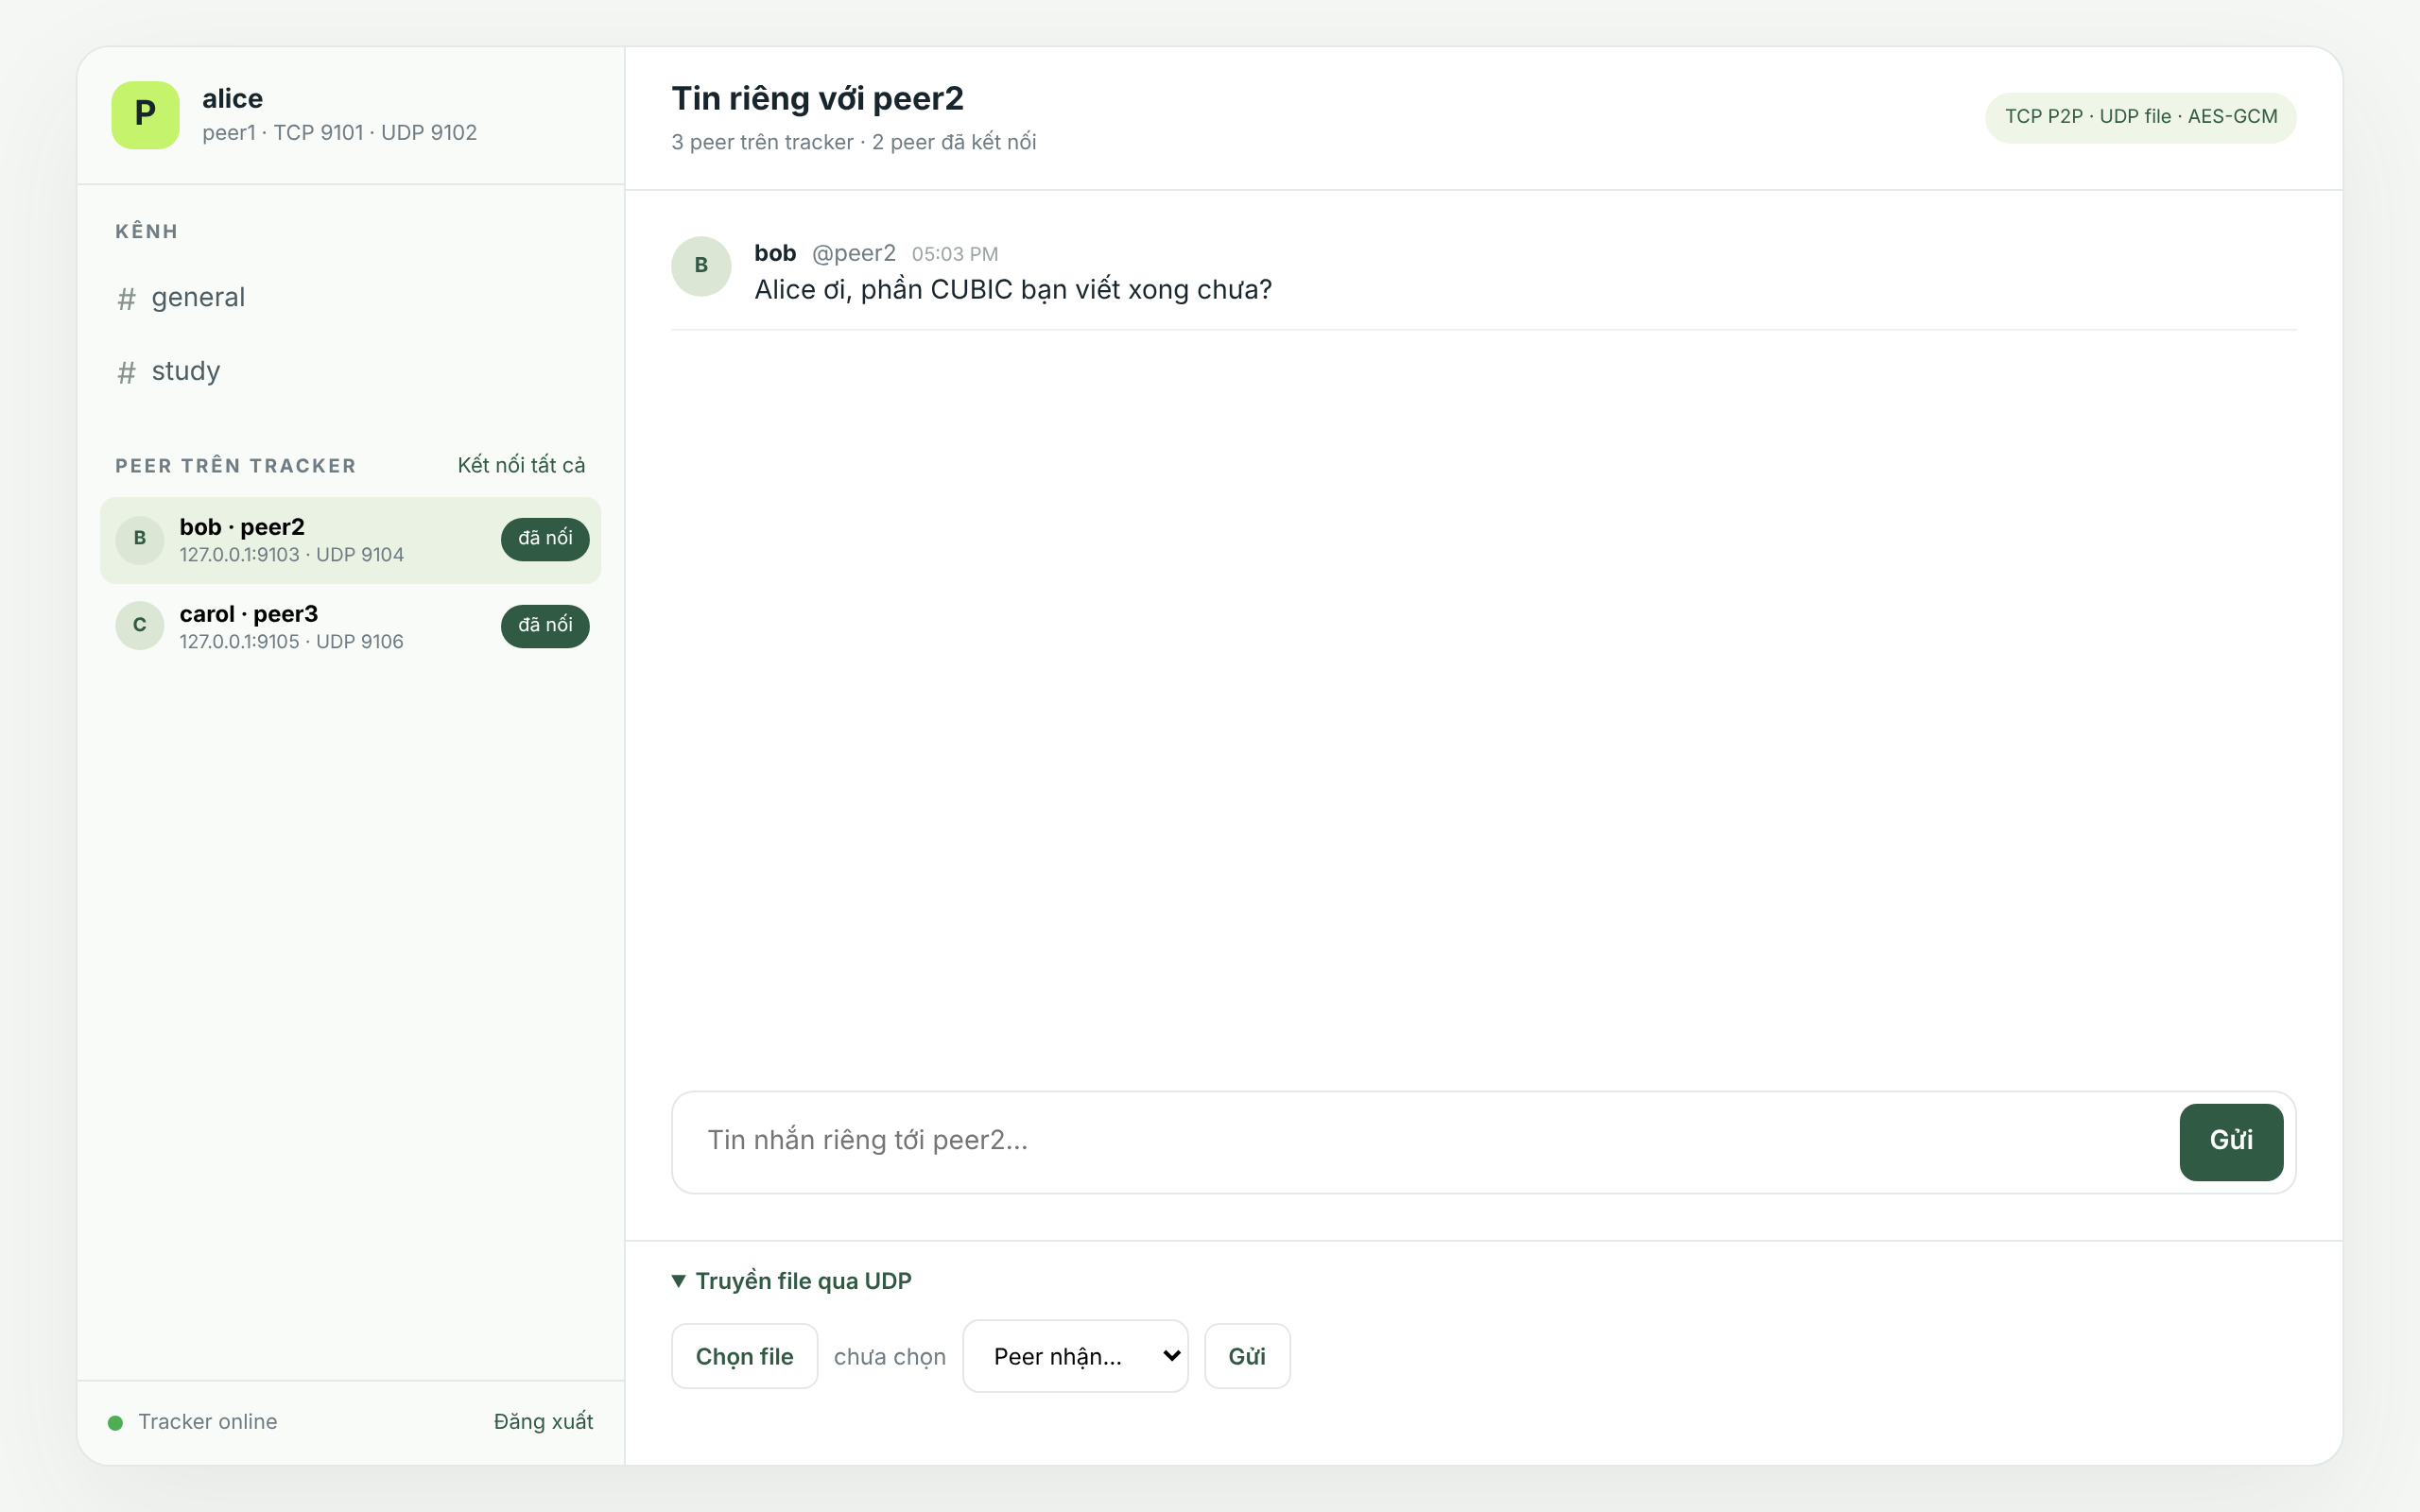
\includegraphics[width=\linewidth]{figures/ui_dm.png}\caption{Direct conversation}\label{fig:ui-dm}
\end{subfigure}\hfill
\begin{subfigure}{0.49\textwidth}\centering
  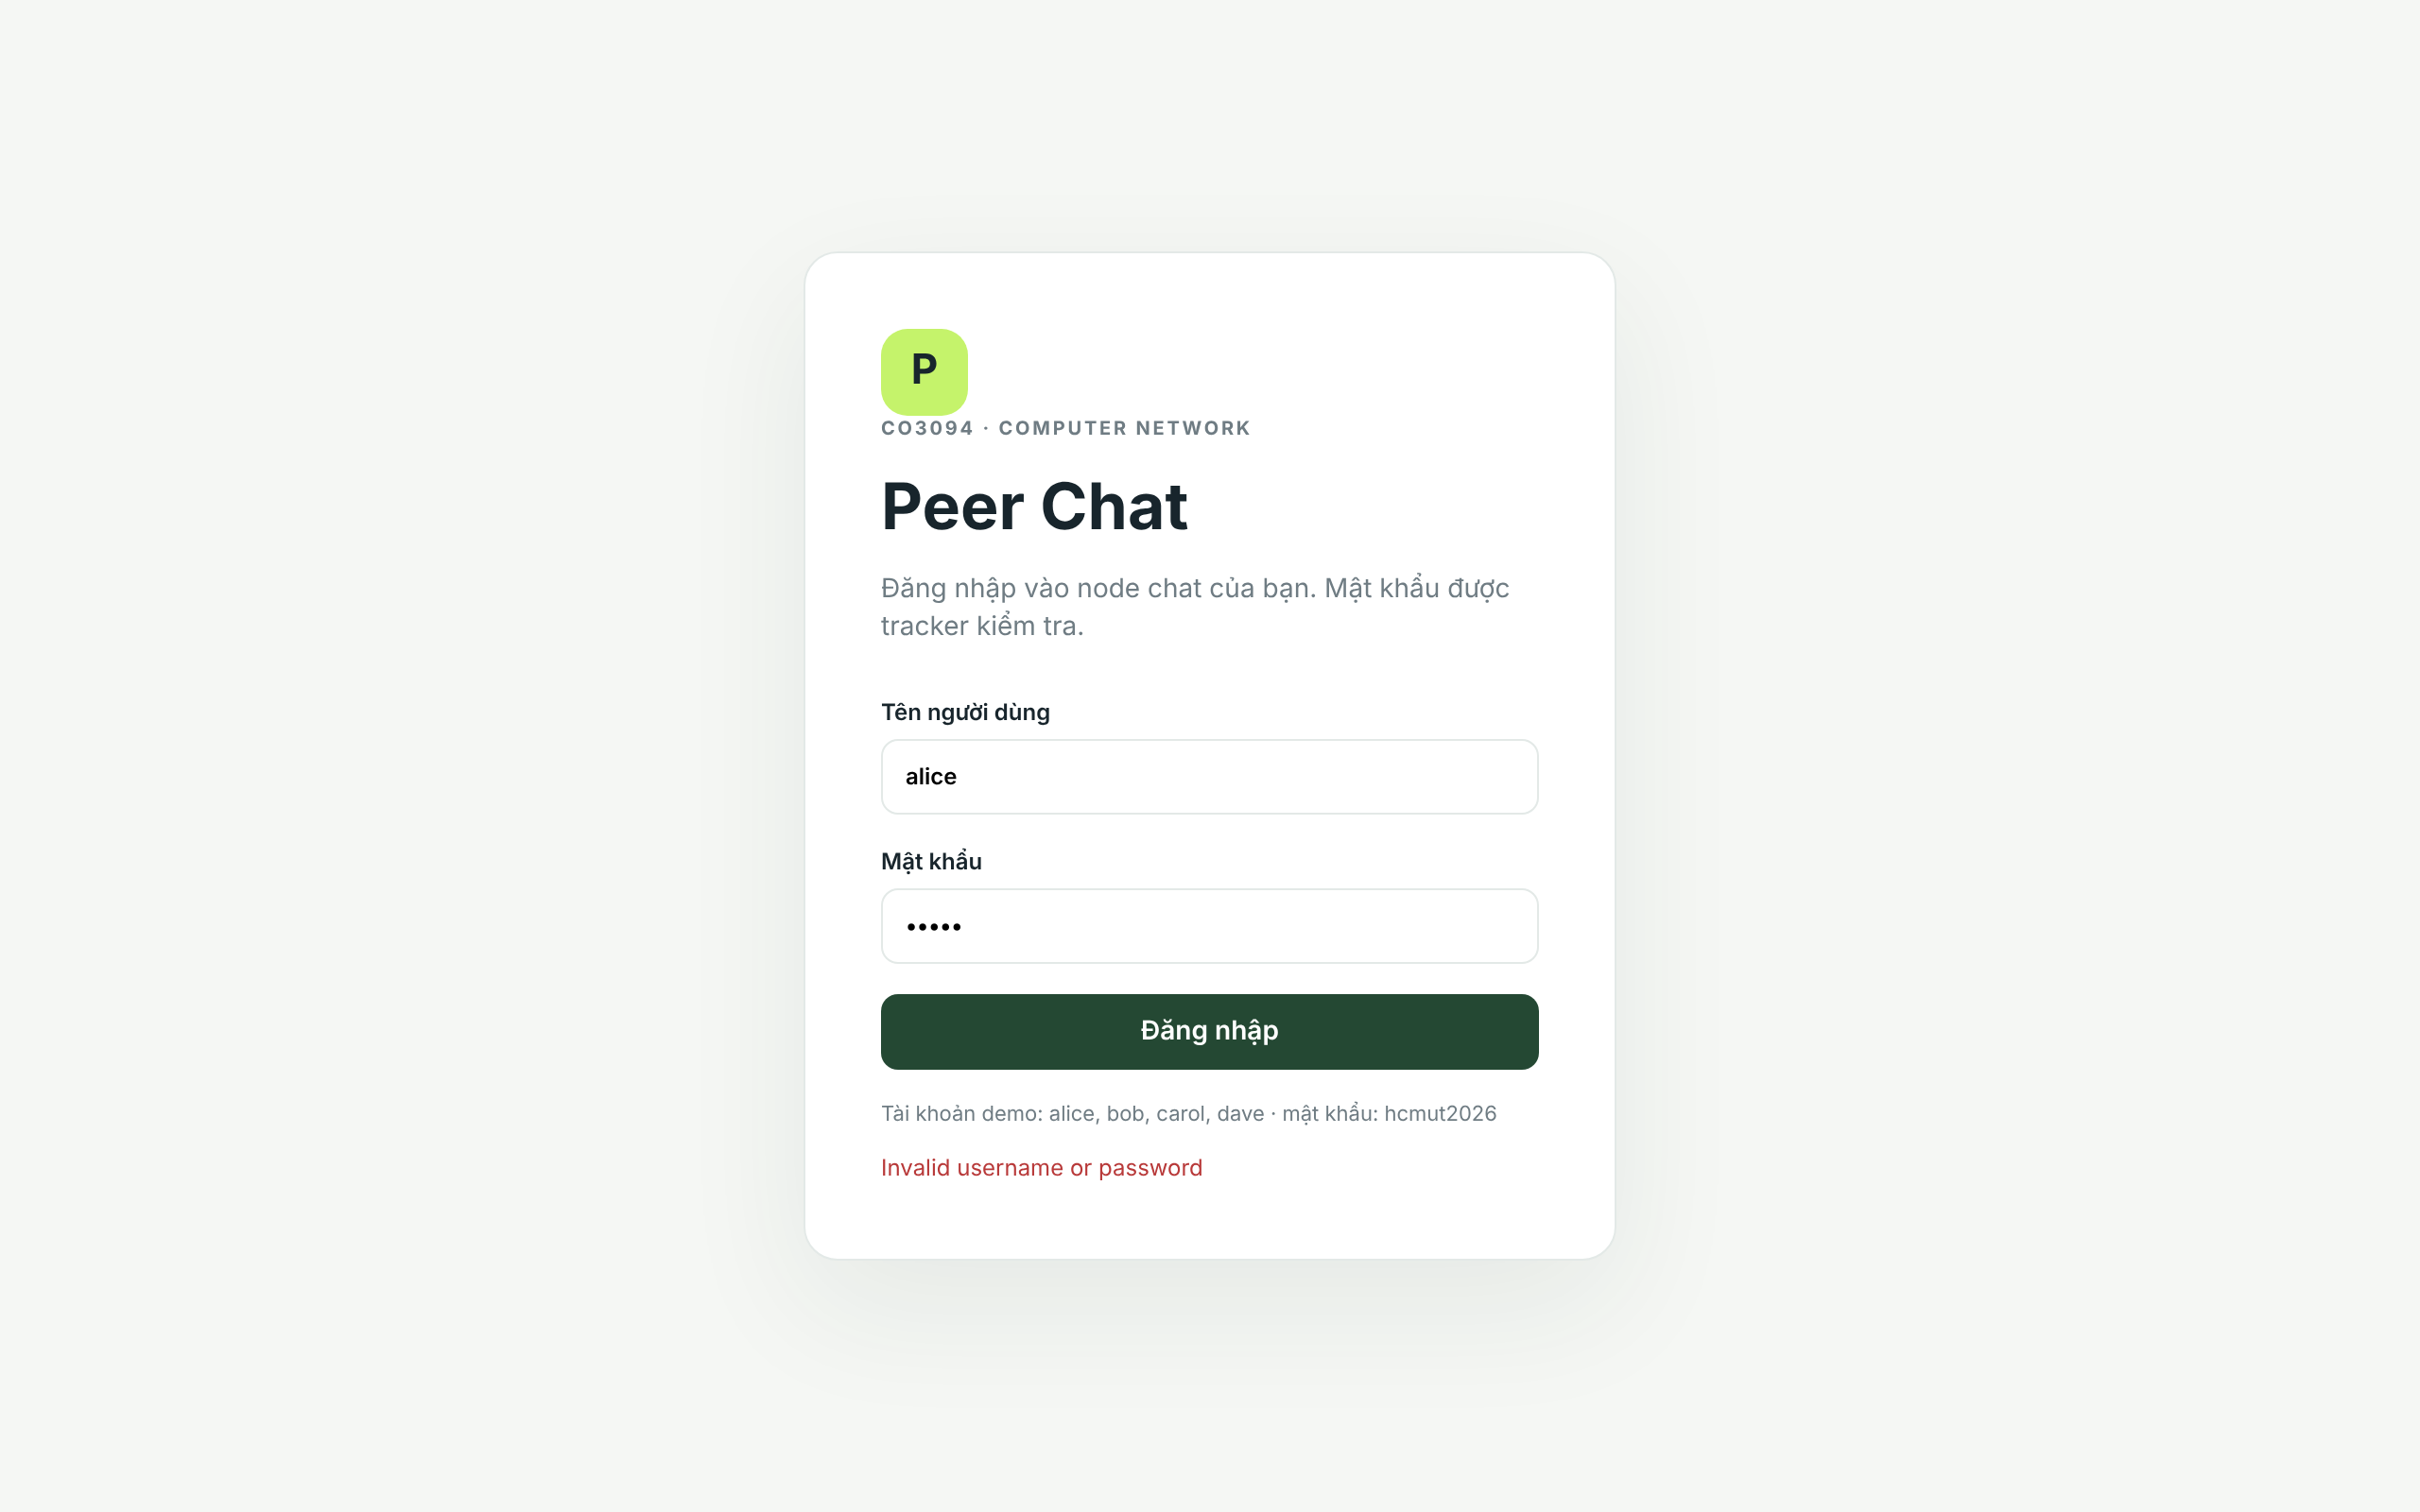
\includegraphics[width=\linewidth]{figures/ui_login_error.png}\caption{Login rejected by the tracker}\label{fig:ui-login}
\end{subfigure}
\caption{Direct messages and login}
\end{figure}

The file panel (\cref{fig:ui-files}) uploads the chosen file to the daemon --- an
\code{XMLHttpRequest} is used because it reports upload progress --- and then shows the UDP transfer
itself: the bar counts acknowledged chunks, and the line below gives the percentage, the size, the
current congestion window and the number of retransmissions, and the throughput when the transfer is
done. The receiver sees an incoming bar and, when the SHA-256 check has passed, a download link.

\begin{figure}[htbp]\centering
\begin{subfigure}{\textwidth}\centering
  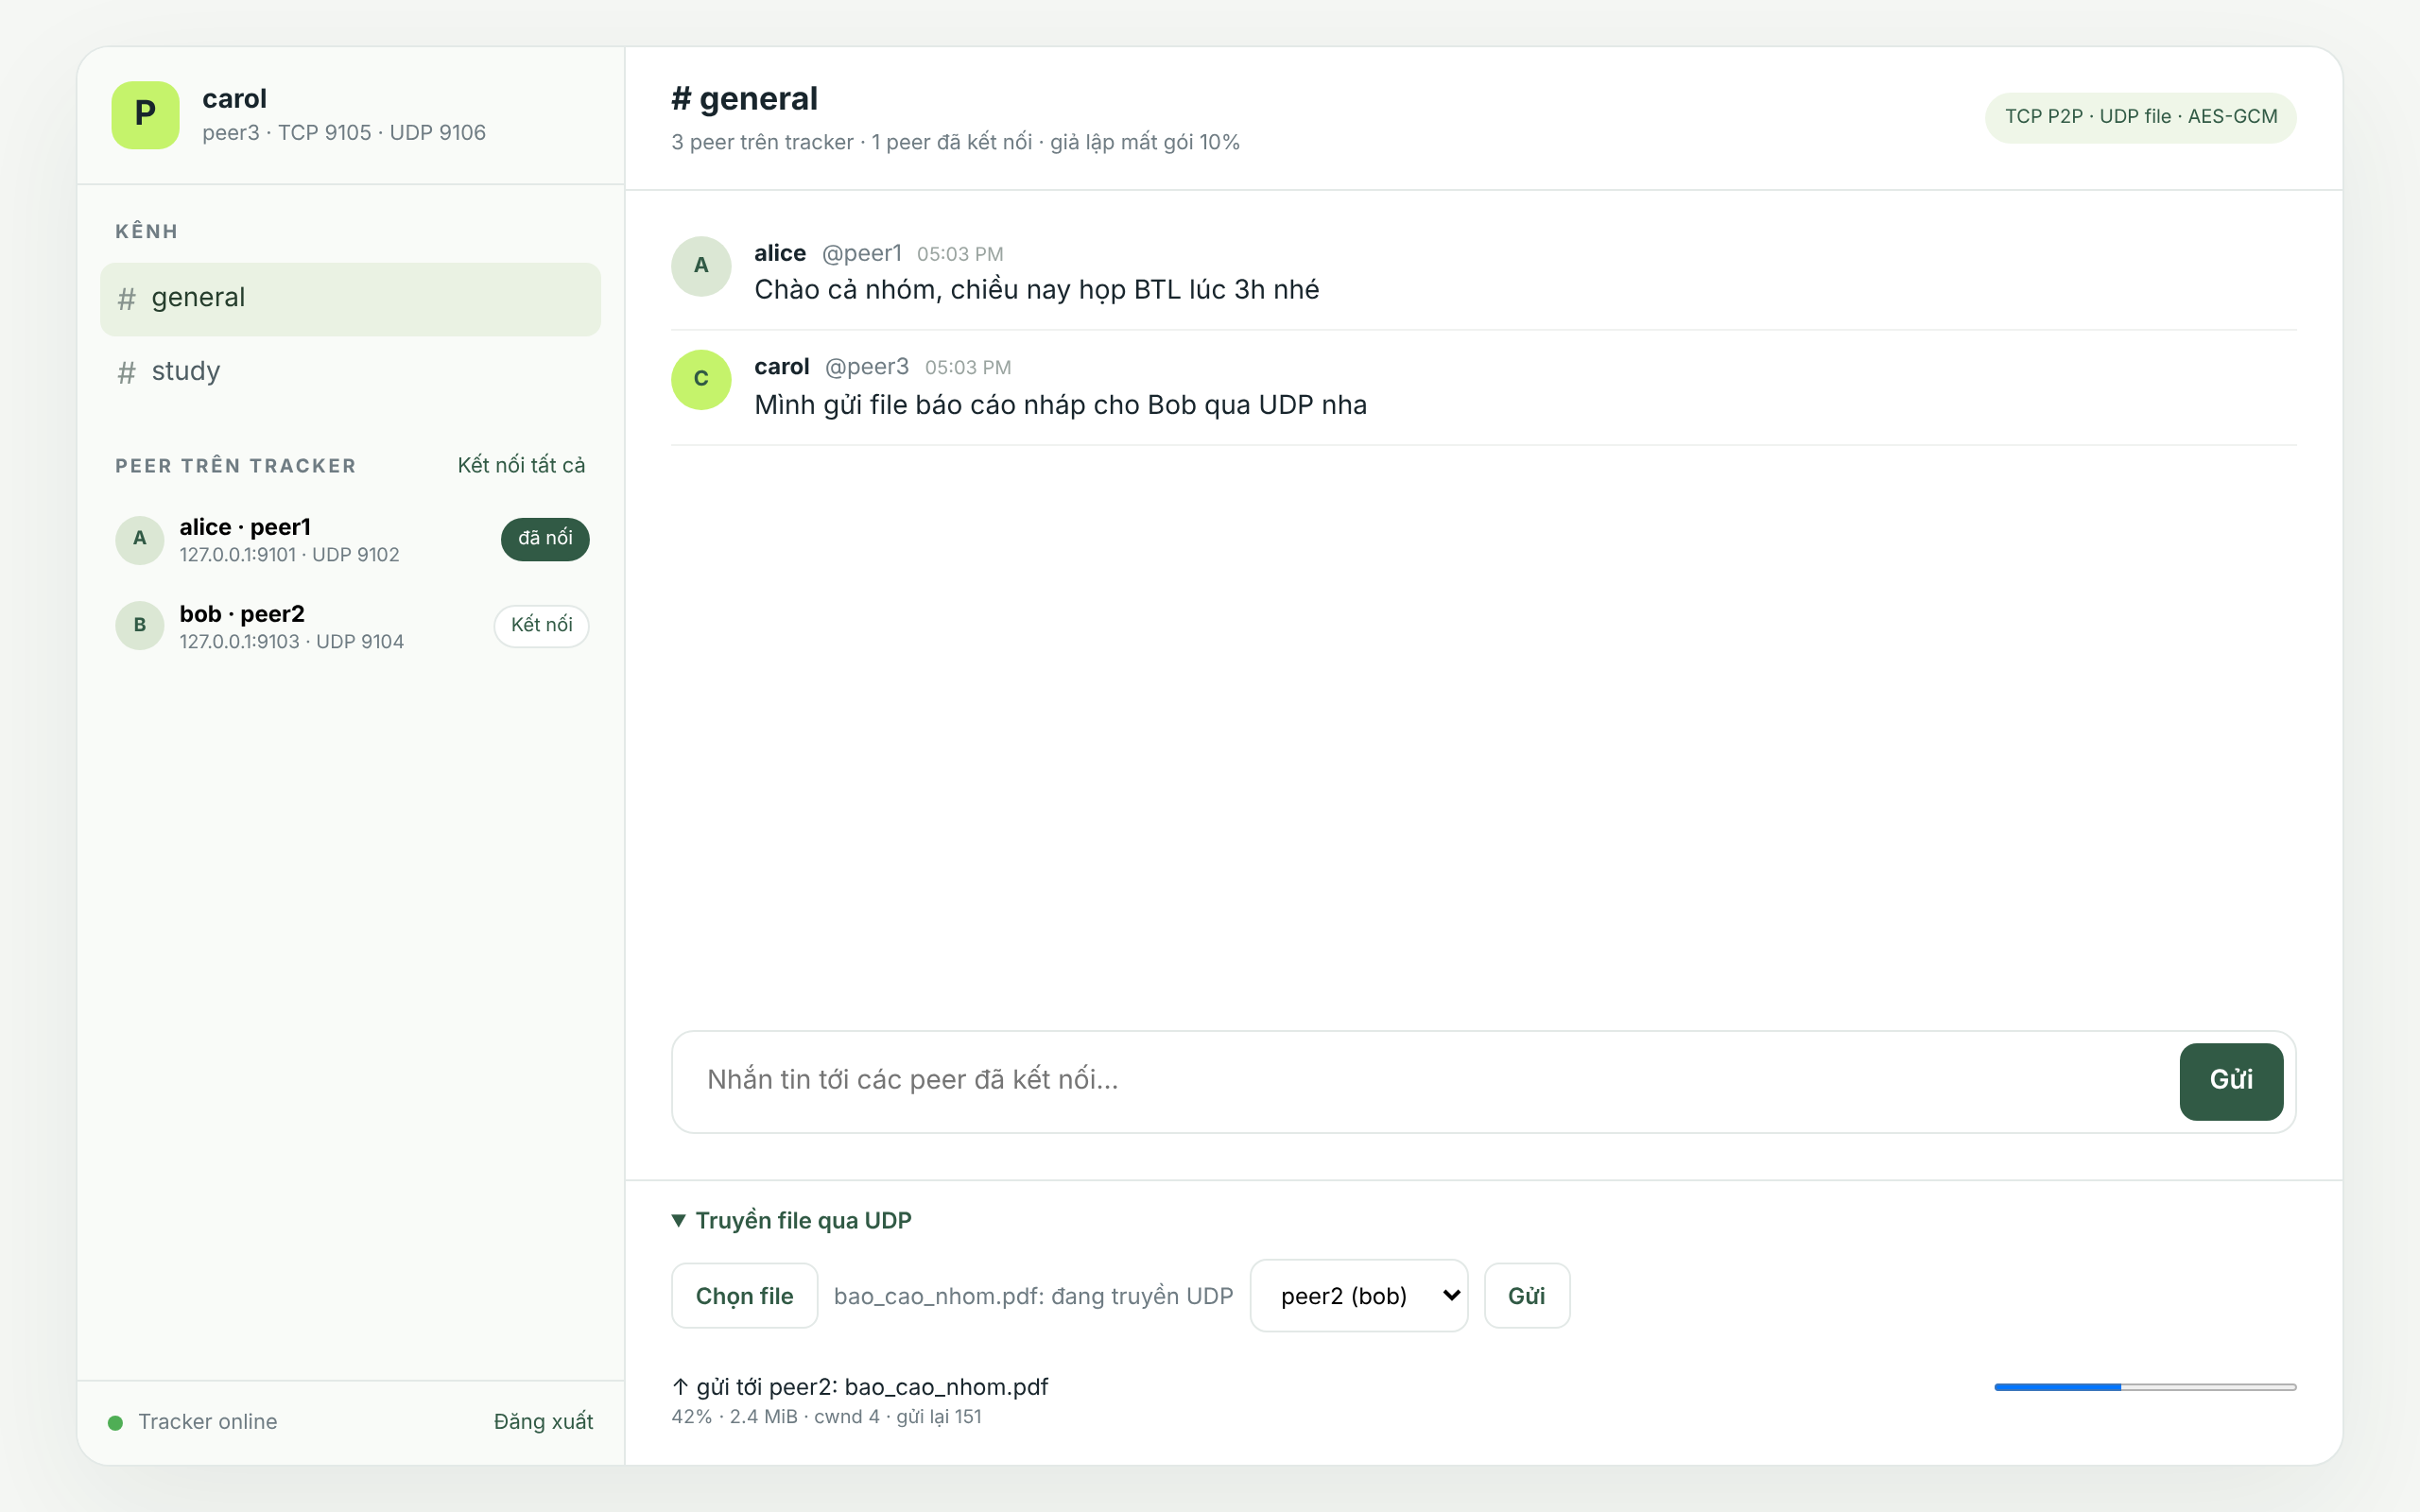
\includegraphics[width=\linewidth, trim=0 0 0 1120, clip]{figures/ui_file_progress.png}
  \caption{Sender during a transfer: 43\,\% acknowledged, \code{cwnd} = 4 after losses}\label{fig:ui-progress}
\end{subfigure}\\[4pt]
\begin{subfigure}{\textwidth}\centering
  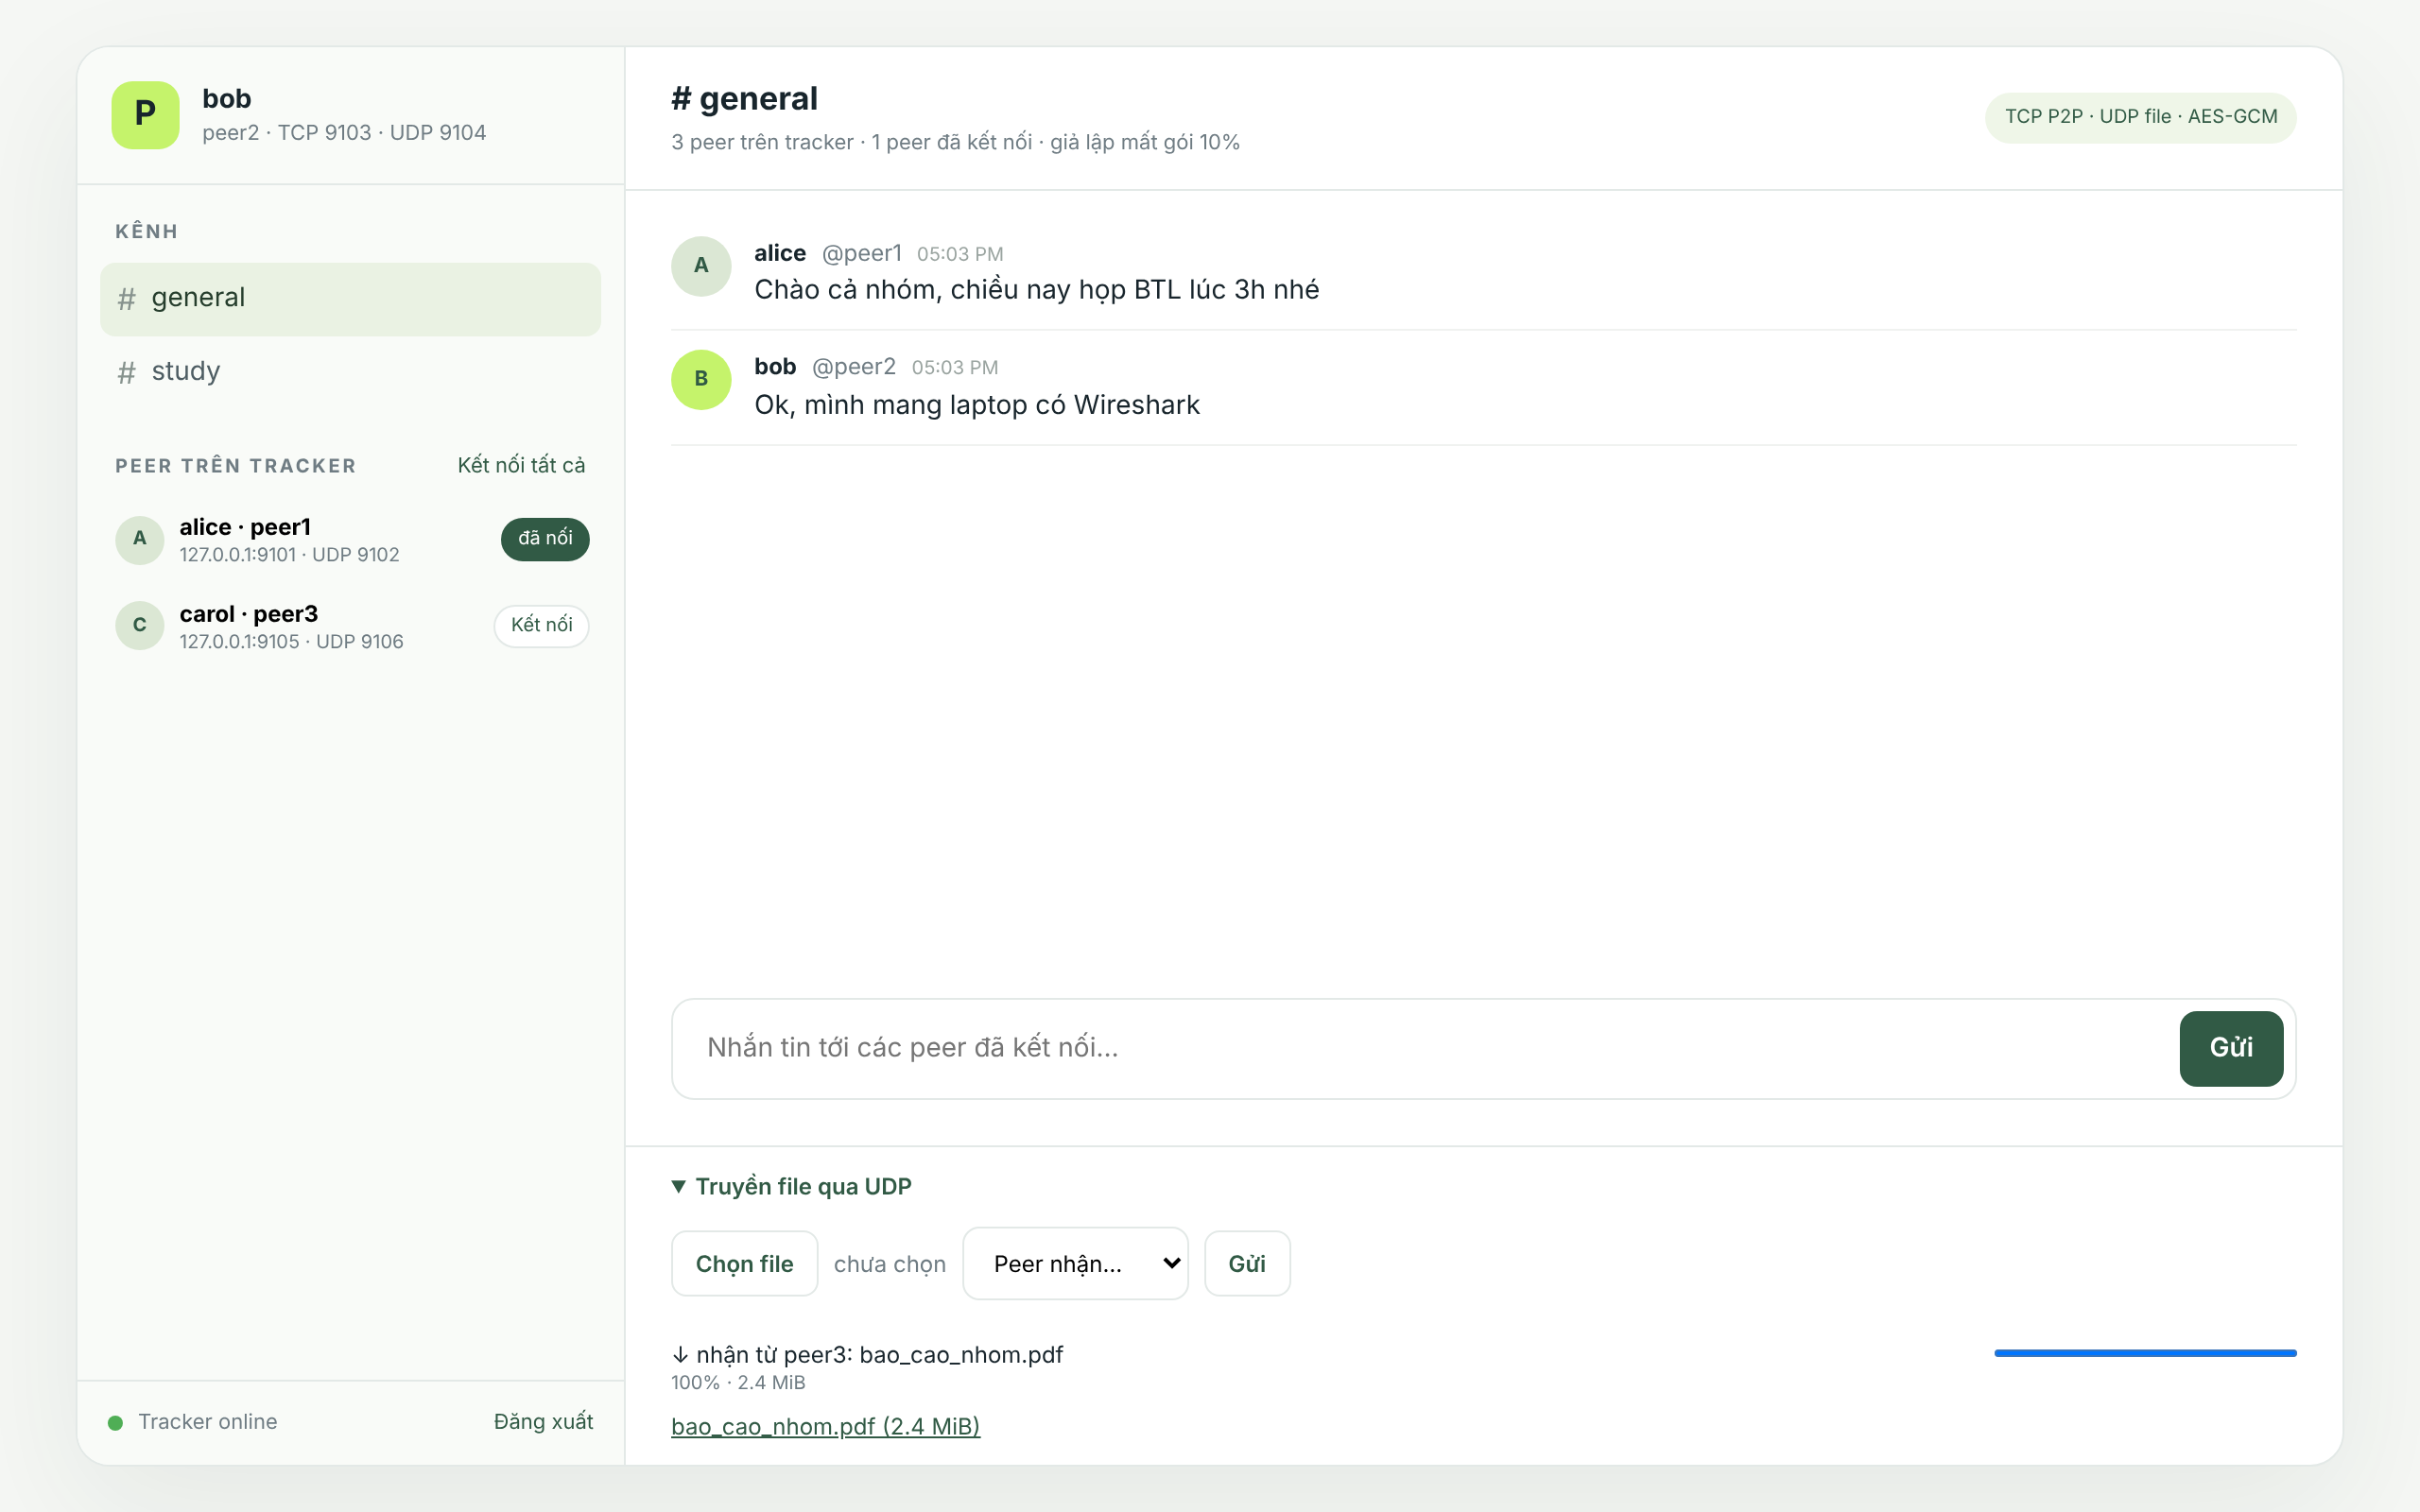
\includegraphics[width=\linewidth, trim=0 0 0 1120, clip]{figures/ui_receiver.png}
  \caption{Receiver: transfer finished, file ready to download}\label{fig:ui-receiver}
\end{subfigure}
\caption{File transfer panel (bottom of the page)}\label{fig:ui-files}
\end{figure}

The tracker serves a small status page with the peers it knows (\cref{fig:ui-tracker}); the
\emph{Seen from} column is the address the tracker observed, which helps to diagnose a wrong
\code{--peer-host} on a LAN.

\fig[fig:ui-tracker]{ui_tracker.png}{Status page of the tracker}{0.75\textwidth}

\section{Testing and Evaluation}\label{sec:testing}

\subsection{Automated tests}
The suite has \FactTests{} tests and uses only \code{unittest} from the standard library. It runs in
25 to 45 seconds, depending on the machine:

\begin{lstlisting}[style=text, caption={Running the tests}, label={lst:run-tests}]
$ python -m unittest discover -s tests -t . -v
...
Ran 69 tests in 25.4s
OK
\end{lstlisting}

The end-to-end tests are the ``local network simulation from several terminal windows'' of rubric
step~10, automated: \code{tests/helpers.py} starts the tracker and each peer as a separate process
with exactly the command a user would type, on free ports, and talks to them over HTTP like a
browser. The whole scenario runs twice, once with asyncio servers and once with one thread per
client. \Cref{tab:tests} summarises what is covered.

\begin{table}[H]\centering\footnotesize
\caption{Test inventory}\label{tab:tests}
\begin{tabularx}{\textwidth}{@{}l r Y@{}}
\toprule
\textbf{File} & \textbf{Tests} & \textbf{What is checked} \\
\midrule
\file{test_protocol.py} & 9 & frames split into single bytes are reassembled; oversized, empty and non-object frames are rejected; changing any AAD field or using another key fails decryption; HMAC on control packets; separate keys per purpose \\
\file{test_tracker.py} & 8 & token ownership (no take-over, no removal without token), user binding, expiry after \SI{45}{s} with a fake clock, heartbeat, salted password hashes, session cookies cannot be forged \\
\file{test_udp_files.py} & 14 & transfer without loss; 20\,\% loss on DATA \emph{and} ACK; empty file; ``\code{../../etc/}'' names; no overwrite; wrong key; receiver errors reach the sender; unreachable receiver; out-of-order and duplicate chunks; invalid chunk count; silent sender is forgotten; tampered chunk; slow start, CUBIC and RTO \\
\file{test_http.py} & 10 & query strings, pseudo-header injection, binary bodies; both server modes with 20 concurrent clients, a handler crash (500) and garbage (400); path traversal; proxy round-robin, fail-over, 404 and 502; configuration parser \\
\file{test_e2e.py} & 28 & login checked by the tracker; user, IP and ports recorded; hijack attempts refused; broadcast only to connected peers; direct messages only to the recipient; validation errors; file over lossy UDP with SHA-256 and download; crashed peer, Ctrl+C, SIGTERM, immediate restart; chat while the tracker is down; 12 peers plus 20 simultaneous registrations; sender verification, duplicates, clock skew, relay fallback \\
\bottomrule
\end{tabularx}
\end{table}

Several tests are regression tests for defects found in the original code (\cref{sec:challenges}):
the swallowed receiver error, transfers that were never forgotten, the cursor based on the sender's
clock, and the peer list that went stale.

\subsection{File transfer under packet loss}
\file{tools/bench_udp.py} sends a \SI{2}{MiB} file (\FactChunks{} chunks) between two endpoints on the
loopback interface and drops the same fraction of datagrams in \emph{both} directions, so DATA and
ACK are both lost. \Cref{tab:bench,fig:bench} give the median of three runs per loss rate.

\begin{table}[H]\centering\small
\caption{UDP file transfer of a 2\,MiB file (2468 chunks) on loopback, median of 3 runs}\label{tab:bench}
\begin{tabular}{@{}rrrrrrrc@{}}
\toprule
\textbf{Loss} & \textbf{Time (s)} & \textbf{KiB/s} & \textbf{Datagrams} & \textbf{Resent} & \textbf{Fast} & \textbf{Timeouts} & \textbf{SHA-256 ok} \\
\midrule
0\,\% & 0.41 & 4,950 & 2468 & 0 & 0 & 0 & yes \\
2\,\% & 0.52 & 3,926 & 2510 & 42 & 36 & 3 & yes \\
5\,\% & 0.85 & 2,421 & 2587 & 119 & 85 & 19 & yes \\
10\,\% & 2.65 & 774 & 2784 & 316 & 145 & 91 & yes \\
20\,\% & 11.57 & 177 & 3320 & 852 & 154 & 312 & yes \\
\bottomrule
\end{tabular}
\end{table}


\fig[fig:bench]{bench_udp.pdf}{Transfer time and number of DATA datagrams versus the loss rate}{\textwidth}

Three observations. First, the file arrived intact in every run --- the protocol is reliable at all
tested loss rates. Second, retransmission is selective: at 20\,\% loss each chunk must be sent
$1/0.8 = 1.25$ times on average just to get through once, i.e.\ about 3085 datagrams for 2468
chunks; the sender needed about 3320, only 8\,\% more than that minimum. Third, time grows much faster
than the number of datagrams: from \FactBenchZero{}\,s without loss to \FactBenchTen{}\,s at 10\,\%
and \FactBenchTwenty{}\,s at 20\,\%. The cause is visible in \cref{fig:cwnd}: without loss the window
reaches its maximum of 64 chunks in a few milliseconds of slow start, while with loss it is cut again
and again and stays between 4 and 15, and every loss that fast retransmit cannot repair costs a
timeout. This is the expected behaviour of a loss-based congestion controller --- it interprets
every loss as congestion --- and the reason why delay-based algorithms such as BBR exist.

\fig[fig:cwnd]{cwnd_trace.pdf}{Congestion window during one transfer at three loss rates}{\textwidth}

The absolute numbers are loopback numbers, measured on a two-core virtual machine: there is no real
link and the round-trip time is below a millisecond, so the limit is the Python code that encrypts,
encodes and parses every datagram (about \FactKibZero{}\,KiB/s without loss). On a real LAN the
round-trip time would make the window matter even more.

\subsection{Manual test on the LAN}
\todo{run the demo on two or three laptops in the same Wi-Fi (README section 3), note the IP
addresses, and add one screenshot of each browser; capture the traffic with Wireshark (filter
\code{tcp.port == 9101 || udp.port == 9102}) and add a screenshot showing that the chat text and file
content are not readable}

\section{Challenges and Solutions}\label{sec:challenges}

The assignment asks for a short reflection on the network problems we met. \Cref{tab:challenges}
lists them; each one is covered by a test.

\begin{table}[H]\centering\footnotesize
\caption{Problems met during development and their solutions}\label{tab:challenges}
\begin{tabularx}{\textwidth}{@{}>{\raggedright\arraybackslash}p{3.6cm} Y Y@{}}
\toprule
\textbf{Problem} & \textbf{Cause} & \textbf{Solution} \\
\midrule
TCP fragmentation: a frame arriving in pieces, or two frames in one read &
TCP is a byte stream; \code{recv} returns whatever has arrived &
length-prefixed frames; the blocking path reads exactly $n$ bytes, the non-blocking path keeps a per-connection buffer and only yields complete frames \\
Every lost ACK caused a needless retransmission &
acknowledgements named only one chunk &
a cumulative field \code{cum} in every ACK, so a later ACK repairs a lost one. A \SI{2.4}{MiB} file with 10\,\% of the ACKs lost: 341 retransmissions before, 0 after \\
Every loss waited for a timer &
the original sender detected loss only with a fixed \SI{0.3}{s} timeout &
fast retransmit after three ACKs above \code{cum}; RTO computed from the measured RTT (RFC~6298) \\
Throughput still collapsed at 10--20\,\% loss &
after a few losses the window fell to two chunks, so a lost chunk could no longer be followed by three later ACKs and every loss waited for the timeout &
a window floor of four chunks and a minimum RTO of \SI{20}{ms} instead of \SI{50}{ms}: \SI{2}{MiB} at 10\,\% loss from \SI{5.9}{s} to \SI{2.7}{s}, at 20\,\% from \SI{36.5}{s} to \SI{11.6}{s} \\
The receiver's error message never reached the sender &
the \code{ValueError} raised for an error ACK was caught by the retry loop's own \code{except ValueError} &
a dedicated \code{TransferError} that the loop does not catch \\
Memory leak on the receiver &
a transfer whose sender died stayed in memory forever &
transfers silent for \SI{30}{s} are discarded with their partial file \\
Large files held several times in memory &
the HTTP body was decoded as text, written to a temporary file, then read back; the receiver kept all chunks in a dictionary &
binary bodies stay bytes; chunks are written to their offset in a \code{.part} file \\
Messages from a peer with a slow clock never appeared &
the browser's cursor was the sender's timestamp &
a local sequence number assigned on arrival \\
A peer that had just joined could not be messaged &
the peer list was refreshed only by the heartbeat &
lookup misses ask the tracker once; a \code{CONNECT} from an unknown peer triggers a refresh in the background \\
Any host could delete or replace a peer at the tracker &
\code{/submit-info} and \code{/remove} trusted the \code{peer_id} in the request &
a peer token, saved on disk so a crashed peer can restart at once \\
The event loop answered 20 slow requests in \SI{2}{s} instead of \SI{0.5}{s} &
asyncio's default executor has only CPUs\,+\,4 threads &
a dedicated pool of 64 threads for blocking handlers \\
\bottomrule
\end{tabularx}
\end{table}

\todo{add the problems you met yourselves while running the demo on real machines (firewall,
\code{--peer-host}, Wi-Fi client isolation, ...)}

\section{Limitations, Future Work and Conclusion}\label{sec:conclusion}

\subsection{Limitations}
\begin{itemize}
  \item \textbf{One shared key per group.} Whoever has it can read every message and could forge a
        sender name; the interface only flags names that do not match the tracker's record.
  \item \textbf{No TLS on HTTP.} The login request from browser to peer and from peer to tracker is
        readable on the network.
  \item \textbf{State in memory.} The tracker forgets who is signed in when it restarts; peers
        re-register automatically but users must sign in again. Message history is kept in memory
        (the last 1000 messages per peer) and is lost when a daemon stops.
  \item \textbf{Simplified CUBIC.} No TCP-friendly region in the strict sense of RFC~8312, no pacing,
        a window of at most 64 chunks, and loss is the only congestion signal.
  \item \textbf{Two fixed channels.} \code{\#general} and \code{\#study}, plus direct conversations;
        no creation of channels, no access control per channel (optional in the brief).
  \item \textbf{One request per HTTP connection} and polling instead of server push; adequate for a
        LAN of a few dozen users.
  \item \todo{anything that did not work in the LAN demo}
\end{itemize}

\subsection{Future work}
\begin{enumerate}
  \item Per-user keys with a key exchange signed by the tracker, so that sender names are proven.
  \item TLS for the HTTP connections (the Python \code{ssl} module wraps the existing sockets).
  \item A delay-based congestion controller (BBR-style pacing) and larger windows for faster links.
  \item Persistent history and user-created channels with membership stored at the tracker.
  \item Persistent TCP connections between peers instead of one connection per message.
\end{enumerate}

\subsection{Conclusion}
The project implements the hybrid model the assignment describes. The tracker does what only a
central server can do --- authenticate users and tell peers where to find each other --- while the
conversation itself and every file go directly from peer to peer, encrypted and authenticated. On
UDP, the application builds its own reliable transport with sequence numbers, selective and
cumulative acknowledgements, a congestion window and fast retransmit, and the measurements show that
it delivers intact files even when a fifth of all datagrams is lost. The design was verified with
\FactTests{} automated tests, most of them against real processes and real sockets.
\todo{one or two sentences on what the team learned}


\clearpage
\bibliographystyle{unsrtnat}
\bibliography{references}

\clearpage
\appendix
\section{Running the Application}\label{app:run}
Python 3.10 or newer and the \code{cryptography} package are required:

\begin{lstlisting}[style=text, caption={Installation and a three-peer demo on one machine}, label={lst:run}]
python -m venv .venv && source .venv/bin/activate      # Windows: .venv\Scripts\activate
python -m pip install -r requirements.txt

python start_tracker.py --server-port 8001                                        # terminal 1
python start_sampleapp.py --server-port 8000 --peer-id peer1 --peer-port 9101 --file-port 9102   # 2
python start_sampleapp.py --server-port 8002 --peer-id peer2 --peer-port 9103 --file-port 9104   # 3
python start_sampleapp.py --server-port 8004 --peer-id peer3 --peer-port 9105 --file-port 9106   # 4
# browsers: http://127.0.0.1:8000, :8002, :8004 (one window per peer); users alice/bob/carol/dave
# add --loss 0.1 to a peer to drop 10 % of its UDP datagrams
\end{lstlisting}

\begin{lstlisting}[style=text, caption={Several machines on one LAN}, label={lst:run-lan}]
python start_tracker.py --server-ip 0.0.0.0 --server-port 8001                    # on 192.168.1.10
python start_sampleapp.py --server-ip 0.0.0.0 --server-port 8000 --peer-id peerA \
    --peer-host <this machine's LAN IP> --peer-port 9101 --file-port 9102 \
    --tracker-url http://192.168.1.10:8001 --shared-key "<group passphrase>"
\end{lstlisting}

\begin{lstlisting}[style=text, caption={Proxy with two static backends}, label={lst:run-proxy}]
python start_backend.py --server-ip 127.0.0.1 --server-port 9000
python start_backend.py --server-ip 127.0.0.1 --server-port 9001
python start_proxy.py --server-ip 127.0.0.1 --server-port 8080          # reads config/proxy.conf
curl -H "Host: app.local" http://127.0.0.1:8080/index.html            # alternates 9000 / 9001
\end{lstlisting}

Other tools: \code{python tools/add_user.py <name>} creates an account (the password is read
without echo and stored as a PBKDF2 hash); \code{python tools/bench_udp.py} repeats the measurement
of \cref{tab:bench}; \code{python report/make_figures.py} regenerates the figures, tables and code
excerpts of this report from the code and the measurements.

\section{API Reference}\label{app:api}

\begin{table}[H]\centering\footnotesize
\caption{Tracker API}\label{tab:api-tracker}
\begin{tabularx}{\textwidth}{@{}l >{\raggedright\arraybackslash}p{5.2cm} Y@{}}
\toprule
\textbf{Route} & \textbf{Request} & \textbf{Response / errors} \\
\midrule
\code{POST /submit-info}, \code{/add-list} & \code{peer_id}, \code{host}, \code{port}, \code{udp_port}, \code{token} (after the first call) & \code{\{ok, token, peers\}}; 400 invalid, 403 id owned by another node \\
\code{GET /get-list} & -- & \code{\{peers: [\{peer_id, username, host, port, udp_port, observed_ip, login_at, registered_at\}]\}} \\
\code{POST /login} & \code{peer_id}, \code{token}, \code{username}, \code{password} & \code{\{ok, username\}}; 401 wrong credentials, 403 wrong token, 404 unknown peer \\
\code{POST /logout} & \code{peer_id}, \code{token} & \code{\{ok\}}; 403, 404 \\
\code{POST /remove} & \code{peer_id}, \code{token} & \code{\{ok\}}; 403 \\
\code{POST /relay}, \code{/broadcast} & \code{peer_id}, \code{token}, \code{targets}, \code{frame} (encrypted \code{CHAT}) & \code{\{ok, delivered, errors\}}; 400 invalid frame, 403 wrong token or origin \\
\code{GET /} & -- & HTML status page \\
\bottomrule
\end{tabularx}
\end{table}

\begin{table}[H]\centering\footnotesize
\caption{Peer API (all routes except login require the session cookie)}\label{tab:api-peer}
\begin{tabularx}{\textwidth}{@{}l >{\raggedright\arraybackslash}p{5.2cm} Y@{}}
\toprule
\textbf{Route} & \textbf{Request} & \textbf{Response} \\
\midrule
\code{POST /login}, \code{/api/login} & \code{username}, \code{password} & \code{\{ok, username, peer_id\}} + \code{Set-Cookie}; 401, 503 tracker down \\
\code{POST /logout}, \code{/api/logout} & -- & cookie cleared \\
\code{GET /api/me} & -- & \code{\{username, peer_id\}} or 401 \\
\code{GET /get-list}, \code{/api/peers} & -- & \code{\{peers, tracker_online\}}, each peer with \code{connected} \\
\code{POST /connect-peer} & \code{peer_id} or \code{all: true} & \code{\{ok, connection\}} or \code{\{ok, results\}}; 404, 502 \\
\code{POST /broadcast-peer} & \code{channel}, \code{text} & \code{\{ok, message, delivery: \{direct, relayed, failed\}\}} \\
\code{POST /send-peer} & \code{peer_id}, \code{text} & same as above \\
\code{POST /api/send} & \code{text} and \code{channel} or \code{peer_id} & same as above \\
\code{GET /api/messages} & query \code{after}, \code{channel} & \code{\{messages\}} with \code{seq} and \code{verified} \\
\code{GET /api/status} & -- & peer id, user, ports, tracker state, connected peers, loss rate \\
\code{POST /api/files/send} & binary body; headers \code{X-Peer-Id}, \code{X-Filename} & 202 \code{\{transfer_id\}}; 404, 413 \\
\code{GET /api/transfers} & -- & progress of every transfer (acked or received chunks, cwnd, retransmissions, status) \\
\code{GET /api/files} & -- & received files with download URLs \\
\code{GET /api/files/download} & query \code{name} & the file as an attachment; 404 \\
\bottomrule
\end{tabularx}
\end{table}

\section{Project Layout}\label{app:layout}
\begin{lstlisting}[style=text, caption={Source tree}, label={lst:tree}]
start_tracker.py  start_sampleapp.py  start_proxy.py  start_backend.py   entry points
apps/       tracker_app.py, chat_app.py (HTTP routes), sampleapp.py (course sample)
chat/       protocol.py (framing, keys, AES-GCM), peer.py (ChatNode, PeerServer),
            udp_files.py (reliable UDP, CUBIC, RTO), tracker.py (registry), accounts.py
daemon/     backend.py (modes), httpadapter.py, request.py, response.py, proxy.py, streaprous.py
static/     chat.html, app.js, chat.css (client side only)
config/     proxy.conf            db/  users.json (PBKDF2 hashes)
tests/      69 tests              tools/  add_user.py, bench_udp.py
report/     this report: latex/, diagrams/ (Mermaid sources), make_figures.py, bench_udp.json
\end{lstlisting}

\section{Further Code Excerpts}\label{app:code}
\pysnippet[lst:register]{tracker_register.py}{Tracker registration with token ownership}
\pysnippet[lst:rtt]{rtt.py}{Retransmission timeout (RFC 6298)}
\pysnippet[lst:proxy]{proxy_policy.py}{Proxy: choosing the backend by policy, with fail-over order}


\ifdraft
\clearpage
\section*{Draft status}
Open \texttt{TODO} markers: \thetodos.
\fi
\end{document}
